\documentclass[11pt,final,fleqn]{article}\usepackage[]{graphicx}\usepackage[]{color}
%% maxwidth is the original width if it is less than linewidth
%% otherwise use linewidth (to make sure the graphics do not exceed the margin)
\makeatletter
\def\maxwidth{ %
  \ifdim\Gin@nat@width>\linewidth
    \linewidth
  \else
    \Gin@nat@width
  \fi
}
\makeatother

\definecolor{fgcolor}{rgb}{0.345, 0.345, 0.345}
\newcommand{\hlnum}[1]{\textcolor[rgb]{0.686,0.059,0.569}{#1}}%
\newcommand{\hlstr}[1]{\textcolor[rgb]{0.192,0.494,0.8}{#1}}%
\newcommand{\hlcom}[1]{\textcolor[rgb]{0.678,0.584,0.686}{\textit{#1}}}%
\newcommand{\hlopt}[1]{\textcolor[rgb]{0,0,0}{#1}}%
\newcommand{\hlstd}[1]{\textcolor[rgb]{0.345,0.345,0.345}{#1}}%
\newcommand{\hlkwa}[1]{\textcolor[rgb]{0.161,0.373,0.58}{\textbf{#1}}}%
\newcommand{\hlkwb}[1]{\textcolor[rgb]{0.69,0.353,0.396}{#1}}%
\newcommand{\hlkwc}[1]{\textcolor[rgb]{0.333,0.667,0.333}{#1}}%
\newcommand{\hlkwd}[1]{\textcolor[rgb]{0.737,0.353,0.396}{\textbf{#1}}}%
\let\hlipl\hlkwb

\usepackage{framed}
\makeatletter
\newenvironment{kframe}{%
 \def\at@end@of@kframe{}%
 \ifinner\ifhmode%
  \def\at@end@of@kframe{\end{minipage}}%
  \begin{minipage}{\columnwidth}%
 \fi\fi%
 \def\FrameCommand##1{\hskip\@totalleftmargin \hskip-\fboxsep
 \colorbox{shadecolor}{##1}\hskip-\fboxsep
     % There is no \\@totalrightmargin, so:
     \hskip-\linewidth \hskip-\@totalleftmargin \hskip\columnwidth}%
 \MakeFramed {\advance\hsize-\width
   \@totalleftmargin\z@ \linewidth\hsize
   \@setminipage}}%
 {\par\unskip\endMakeFramed%
 \at@end@of@kframe}
\makeatother

\definecolor{shadecolor}{rgb}{.97, .97, .97}
\definecolor{messagecolor}{rgb}{0, 0, 0}
\definecolor{warningcolor}{rgb}{1, 0, 1}
\definecolor{errorcolor}{rgb}{1, 0, 0}
\newenvironment{knitrout}{}{} % an empty environment to be redefined in TeX

\usepackage{alltt}

% basic packages
\usepackage[T1]{fontenc}
\usepackage[margin=1in] { geometry }
\usepackage{amssymb,amsmath, bm}
\usepackage{verbatim}
\usepackage[latin1]{inputenc}
%\usepackage[OT1]{fontenc}
\usepackage{setspace}
\usepackage{natbib}
\usepackage{enumitem}
\usepackage[hyphens,spaces,obeyspaces]{url}
\usepackage[font={bf}]{caption}
%\usepackage{pgfplots}
%\usepackage[font={bf}]{caption}
\usepackage{latexsym}
%\usepackage{euscript}
\usepackage{graphicx}
\usepackage{marvosym}
%\usepackage[varg]{txfonts}  Older version of ``g'' in math.
\usepackage{pdflscape}
\usepackage{algorithm}

% bibliography packages
\usepackage{natbib}
\bibpunct{(}{)}{;}{a}{}{,}
\bibliographystyle{apa}
\renewcommand{\bibname}{References}

% hyperref options
\usepackage{color}
\usepackage{hyperref}
\usepackage{xcolor}
\hypersetup{
    colorlinks,
    linkcolor={blue!50!black},
    citecolor={blue!50!black},
    urlcolor={blue!80!black}
}
\newcommand*{\Appendixautorefname}{Appendix}
\renewcommand*{\sectionautorefname}{Section}
\renewcommand*{\subsectionautorefname}{Section}
\renewcommand*{\subsubsectionautorefname}{Section}
\newcommand{\subfigureautorefname}{\figureautorefname}
\newcommand{\aref}[1]{\hyperref[#1]{Appendix~\ref{#1}}}
\newcommand{\algorithmautorefname}{Algorithm}

% packages for tables
\usepackage{longtable}
\usepackage{booktabs, threeparttable}
\usepackage{threeparttablex}
\usepackage{tabularx}
% dcolumn package
\usepackage{dcolumn}
\newcolumntype{.}{D{.}{.}{-1}}
\newcolumntype{d}[1]{D{.}{.}{#1}}
\captionsetup{belowskip=10pt,aboveskip=-5pt}
\usepackage{multirow}
% rotating package
\usepackage[figuresright]{rotating}
\usepackage{pdflscape}
\usepackage{subcaption}
\usepackage{caption} 
\captionsetup[table]{skip=5pt}

% packages for figures
\usepackage{grffile}
\usepackage{afterpage}
\usepackage{float}
\usepackage[section]{placeins}
\usepackage[export]{adjustbox}

% theorem package
\usepackage{theorem}
\theoremstyle{plain}
\theoremheaderfont{\scshape}
\newtheorem{theorem}{Theorem}
\newtheorem{assumption}{Assumption}
\newtheorem{lemma}{Lemma}
\newtheorem{proposition}{Proposition}
\newtheorem{remark}{Remark}
\newcommand{\qed}{\hfill \ensuremath{\Box}}
\newcommand\indep{\protect\mathpalette{\protect\independenT}{\perp}}
\DeclareMathOperator{\sgn}{sgn}
\DeclareMathOperator{\tr}{tr}
\DeclareMathOperator{\argmin}{arg\min}
\DeclareMathOperator{\argmax}{arg\max}
\def\independenT#1#2{\mathrel{\rlap{$#1#2$}\mkern2mu{#1#2}}}
\providecommand{\norm}[1]{\lVert#1\rVert}
\renewcommand\r{\right}
\renewcommand\l{\left}
\newcommand\E{\mathbb{E}}
\newcommand\dist{\buildrel\rm d\over\sim}
\newcommand\iid{\stackrel{\rm i.i.d.}{\sim}}
\newcommand\ind{\stackrel{\rm indep.}{\sim}}
\newcommand\cov{{\rm Cov}}
\newcommand\var{{\rm Var}}
\newcommand\SD{{\rm SD}}
\newcommand\bone{\mathbf{1}}
\newcommand\bzero{\mathbf{0}}
\newcommand\logit{{\rm logit}}

% file paths and definitions
\makeatletter
\newcommand*\ExpandableInput[1]{\@@input#1 }
\makeatother

% spacing 
\usepackage[compact]{titlesec}
\setlength{\parindent}{0pt}
\setlength{\parskip}{6pt plus 2pt minus 1pt}
\setstretch{1}

% appendix settings
\usepackage[toc,page,header]{appendix}
\renewcommand{\appendixpagename}{\centering Appendices}
\usepackage{chngcntr}
\usepackage{etoolbox}
\usepackage{lipsum}

% new commands
\newcommand\CPP{{C\texttt{++}}}
\newcommand\R{{\textsf{R}}}
\newcommand*\sameaff[1][\value{footnote}]{\footnotemark[#1]}
\newcommand\floor[1]{\lfloor#1\rfloor}
\newcommand\ceil[1]{\lceil#1\rceil}

% title
\title{A Description of the IVI-RA Model v0.1}
\author{Devin Incerti\footnote{\href{http://www.thevalueinitiative.org/}{Innovation and Value Initiative}} \and Jeroen P. Jansen\sameaff}
\date{\today}
\IfFileExists{upquote.sty}{\usepackage{upquote}}{}
\begin{document}
\maketitle

\begingroup
 \hypersetup{linkcolor=black} \tableofcontents
 \listoffigures
 \listoftables
\endgroup



\section{Overview}\label{overview}

This document describes version 0.1 of the Innovation and Value Initiative's (IVIs) rheumatoid arthritis (RA) cost-effectiveness model. The IVI-RA model is an individual patient simulation (IPS) that simulates patients one at a time. The model can be run with multiple perspectives (e.g., health care sector, societal) and accounts for both parameter and structural uncertainty. Since the range of defendable scientific approaches is large, the IVI-RA model consists of 336 possible model structures. Structural uncertainty can be quantified by estimating cost-effectiveness across these different model structures and parameter uncertainty is quantified using probabilistic sensitivity analysis (PSA). 

The model is available as an \href{https://cran.r-project.org/}{\R{}} package with documentation available \href{https://innovationvalueinitiative.github.io/IVI-RA/index.html}{online}. The source code can be viewed or downloaded at our \href{https://github.com/InnovationValueInitiative/IVI-RA}{GitHub repository}. The IPS was primarily written in \CPP{} so that PSA and analyses of structural uncertainty can be run in a reasonable amount of time. The model can either be run using \R{} (see \href{https://innovationvalueinitiative.github.io/IVI-RA/index.html}{documentation}) or \href{http://www.shinyapps.io/}{online} with our user-friendly R Shiny web application. 

This document is structured as follows. We begin by discussing treatment strategies that can be modeled in \autoref{sec:treatments}. \autoref{sec:model-structures} outlines the competing model structures. \autoref{sec:populations} examines the data needed to define a population and run an analysis. \autoref{sec:data-parameters} describes the statistical techniques used to estimate the model parameters and the data sources used. \autoref{sec:sim-uncertainty} details the simulation techniques used to implement the IVI-RA model and quantify uncertainty. \autoref{sec:validation} focuses on methods for validating the model. Lastly, \autoref{sec:limitations} discusses limitations and areas for improvement. 

\section{Treatment strategies}\label{sec:treatments}
The primary purpose of the model is to evaluate the cost-effectiveness of treatments for rheumatoid arthritis (RA). Since patients typically use multiple treatments over a lifetime, the model is capable of simulating a treatment sequence of any arbitrary length. Treatments that can be included in a sequence include conventional disease-modifying anti-rheumatic drugs (cDMARDs) such as methotrexate as well as the following biologic DMARDs (bDMARDs):

\begin{itemize}
\item \textbf{Tumor necrosis factor (TNF) inhibitors}: etanercept, adalimumab, infliximab, certolizumab, golimumab
\item \textbf{non-TNF inhibitors}: abatecept, tocilizumab, rituximab
\item \textbf{Janus kinase/signal transducers and activators of transcription (JAK/STAT) inhibitors}: tofacitinib
\end{itemize}

At the end of a sequence, patient switch to non-biologic therapy (NBT), which encompasses a range of therapies that clinicians may feel is appropriate for all patients such as methotrexate and sulfasalazine \citep{stevenson2016adalimumab, stevenson2017cost}.

\section{Competing model structures}\label{sec:model-structures}
The IVI-RA model is a discrete-time IPS with 6 month cycles that can be run using a number of different model structures. Like most RA cost-effectiveness models, the model measures changes in disease severity using the Health Assessment Questionnaire (HAQ) Disability Index score \citep{tosh2011sheffield, carlson2015economic, stephens2015modelling, stevenson2016adalimumab, icer2017tim, stevenson2017cost}. In particular, at the start of the simulation, each patient is assigned a baseline HAQ score. Subsequently, the impact of the disease measured by the HAQ trajectory over time is modeled as a function of a sequence of treatments (\autoref{fig:haq-structure}). In the absence of treatment, HAQ deteriorates at a certain rate as depicted by the dashed line in the figure. Treatment is separated into two distinct phases: an initial phase of up to 6 months, consistent with data reported from randomized controlled trials (RCTs), and a maintenance phase thereafter until discontinuation. 

\begin{figure}
\centering
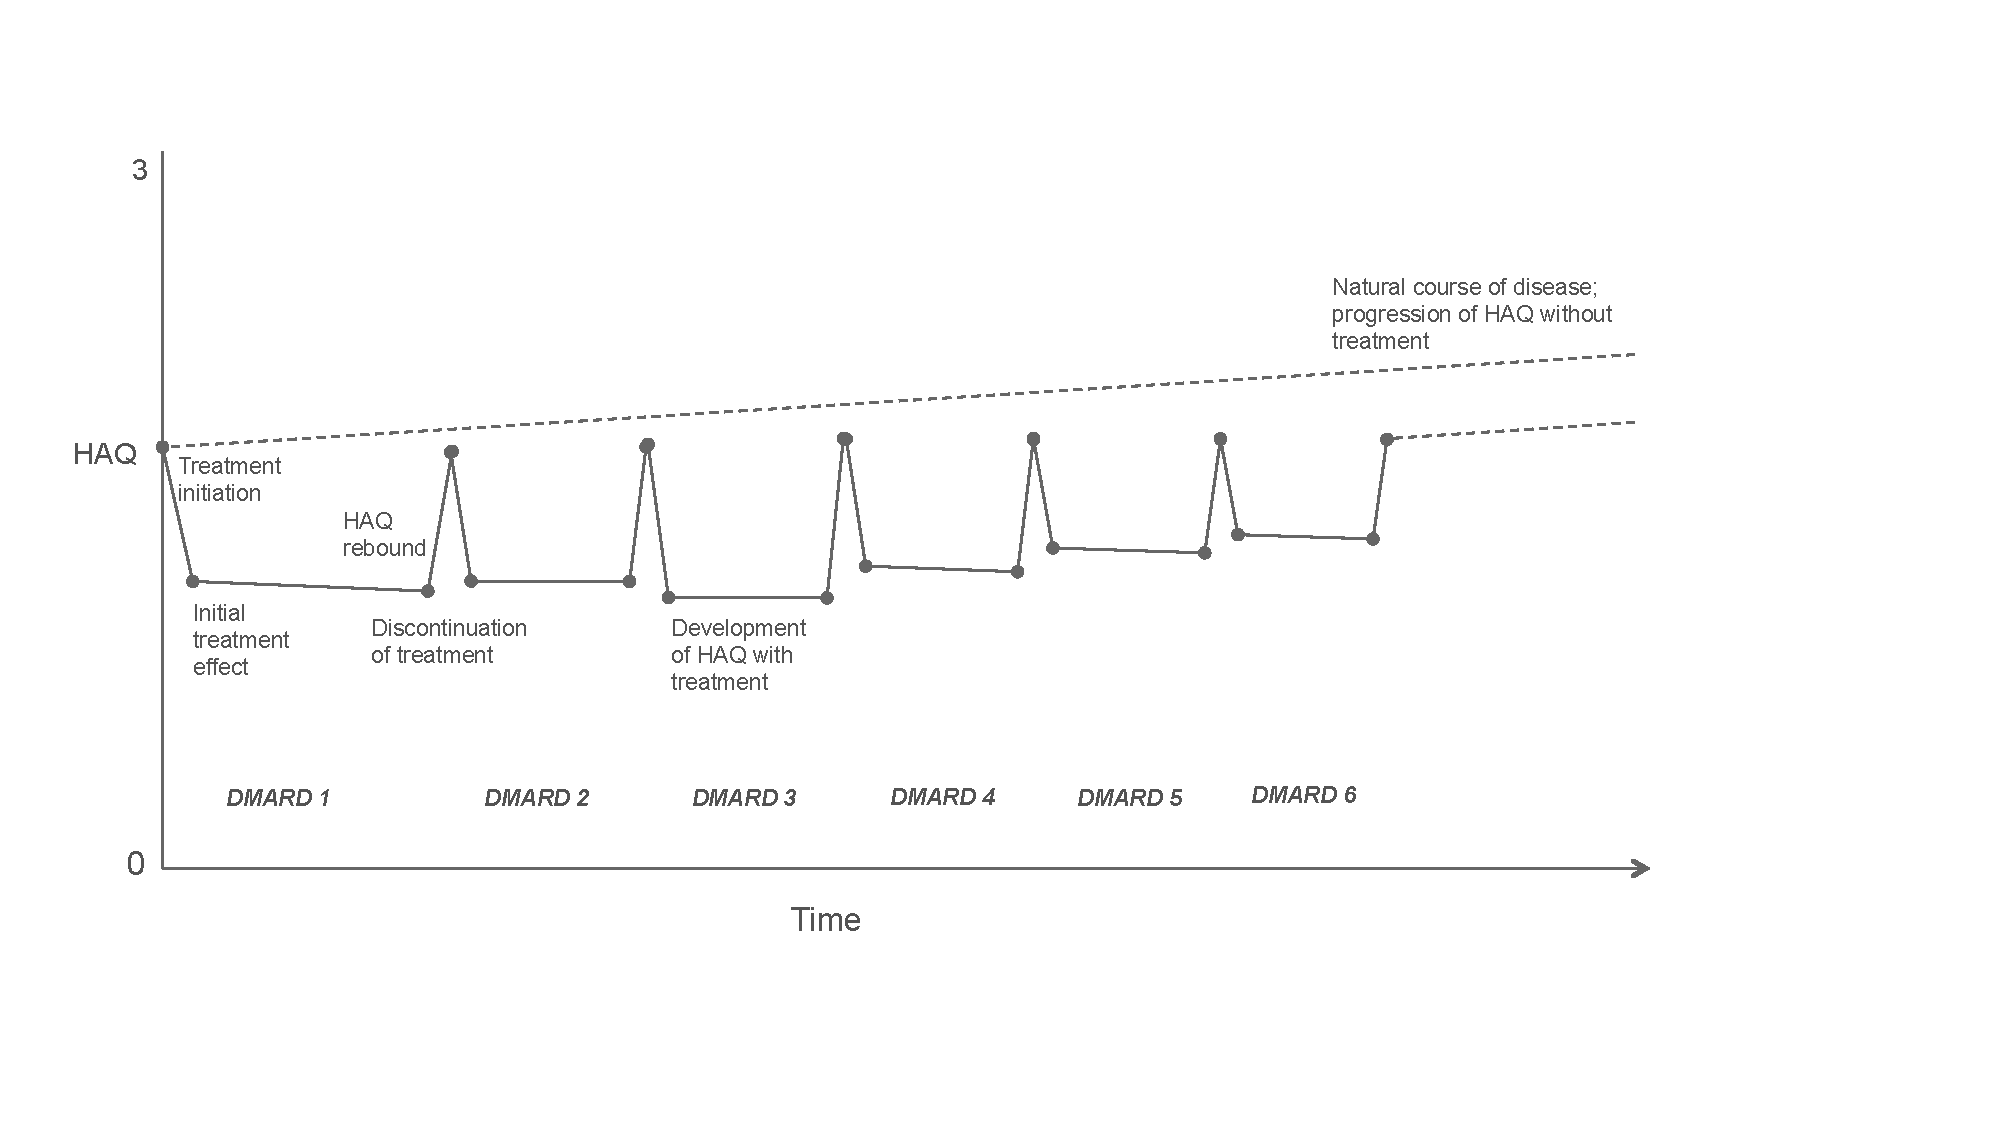
\includegraphics[max size={\textwidth}{\textheight}]{haq-structure.pdf}
\caption{Model structure regarding development of HAQ with sequential
biologic treatment}\label{fig:haq-structure}
\end{figure}

During the initial treatment phase HAQ is modeled as a change from baseline. Three possible model structures labeled \textbf{H1-H3} are possible. 

\begin{itemize}
\item \textbf{H1}: Treatment $\rightarrow$ ACR $\rightarrow$ HAQ
\item \textbf{H2}: Treatment $\rightarrow$ ACR $\rightarrow$ EULAR $\rightarrow$ HAQ
\item \textbf{H3}: Treatment $\rightarrow$ HAQ
\end{itemize}

In \textbf{H1}, treatment influences HAQ through its effect on the American College of Rheumatology (ACR) response criteria, which is similar to the structure used in other US based cost-effectiveness models \citep[e.g.][]{carlson2015economic, icer2017tim}. ACR 20/50/70 response is defined as at least a 20/50/70\% improvement. In the simulation, we convert these overlapping ACR categories to four mutually exclusive categories: no response (defined as less than 20\% improvement), ACR 20\% to <50\% improvement, ACR 50\% to <70\% improvement, and ACR 70\% improvement or greater. The rationale for using ACR response rather than HAQ directly is that the evidence base relating treatment to ACR response is larger than the evidence based relating treatment to HAQ. \textbf{H2} follows the National Institute for Health and Care Excellence (NICE) cost-effectiveness model \citep{stevenson2016adalimumab, stevenson2017cost} and models the effect of treatment on HAQ indirectly through its effect on ACR response and, in turn, the three categories of the European League Against Rheumatism (EULAR) response (no response, moderate response, or good response). Finally, since modeling the effect of treatment on HAQ through intermediary variables may mediate treatment response, in \textbf{H3}, treatment impacts HAQ directly.

Treatment switching during the initial treatment phase is modeled using 6 possible structures labeled \textbf{S1-S6}.

\begin{itemize}
\item \textbf{S1:} Treatment $\rightarrow$ ACR $\rightarrow$ Switch
\item \textbf{S2:} Treatment $\rightarrow$ ACR $\rightarrow$ $\Delta$DAS28 $\rightarrow$ DAS28 $\rightarrow$ Switch 
\item \textbf{S3:} Treatment $\rightarrow$ ACR $\rightarrow$ $\Delta$SDAI $\rightarrow$ SDAI $\rightarrow$ Switch 
\item \textbf{S4:} Treatment $\rightarrow$ ACR $\rightarrow$ $\Delta$CDAI $\rightarrow$ CDAI $\rightarrow$ Switch 
\item \textbf{S5:} Treatment $\rightarrow$ $\Delta$DAS28 $\rightarrow$ DAS28 $\rightarrow$ Switch 
\item \textbf{S6:} Treatment $\rightarrow$ ACR $\rightarrow$ EULAR $\rightarrow$ Switch
\end{itemize}

\textbf{S1} follows a common approach where ACR non-responders discontinue treatment \citep[e.g.][]{carlson2015economic, icer2017tim}. One drawback of this approach is that it is not consistent with current treat-to-target guidelines in the United States \citep{singh20162015}. In \textbf{S2-S5}, treatment switching consequently depends on disease activity (remission, low, moderate, high) \citep{anderson2012rheumatoid}. In \textbf{S2-S4}, ACR response predicts the change in disease activity from baseline, which along with baseline disease activity, predicts absolute disease activity. Patients with moderate or high disease switch treatment while patients with low disease activity or in remission continue treatment. Disease activity is measured using either the Disease Activity Score with 28-joint counts (DAS28) \citep{prevoo1995modified}, Simplified Disease Activity Index (SDAI) \citep{smolen2003simplified, aletaha2005simplified}, or the Clinical Disease Activity Index (CDAI) \citep{aletaha2005acute}. 

\textbf{S5} is similar to \textbf{S2-S4}, but models the effect of treatment on changes in DAS28 directly, rather than indirectly through ACR response. We also aimed to model the direct effect of treatment on SDAI and CDAI, but sufficient clinical trial data are not available. Finally, since in the UK, the British Society for Rheumatology and the British Health Professionals in Rheumatology recommends using the EULAR response \citep{deighton2010bsr}, treatment switching in \textbf{S6} depends on EULAR response. In particular, following the NICE model, we assume that EULAR non-responders discontinue treatment while moderate and good responders continue treatment \citep{stevenson2016adalimumab}. The reasoning is that rules stipulated by NICE require a DAS28 improvement of more than 1.2 to continue treatment which is associated with moderate or good EULAR response. 

Not all model structures \textbf{S1-S6} can be used with each of \textbf{H1-H3}. If \textbf{H1} is used, then \textbf{S1-S5} are available, but \textbf{S6} is not because EULAR response is not simulated. In \textbf{H2}, \textbf{S1-S6} are all available while in \textbf{H3} only \textbf{S5} can be used since ACR response is not simulated. The 12 possible model structures and the number of each structure are outlined in \autoref{tbl:initial-model-structure}.  

\begin{table}[!ht] 
\begin{center}
\begin{threeparttable}
\caption{Model structures for initial treatment phase} \label{tbl:initial-model-structure}
\begin{tabularx}{\textwidth}{@{\extracolsep{\fill}}lcccccc}
\hline
\multicolumn{1}{l}{} & \multicolumn{1}{c}{S1} & \multicolumn{1}{c}{S2} & \multicolumn{1}{c}{S3} & \multicolumn{1}{c}{S4} & \multicolumn{1}{c}{S5} & \multicolumn{1}{c}{S6}  \\
\hline
H1 & 1 & 2 & 3 & 4 & 5 & - \\
H2 & 6 & 7 & 8 & 9 & 10 & 11 \\
H3 & - & - & - & - & 12  & -\\
\hline
\end{tabularx}
\scriptsize
Notes: Rows denote the model structure used to relate treatment to HAQ and columns denote the model structure used to determine treatment switching. Each number denotes a unique model structure (i.e., 1 corresponds to H1 and S1, and 8 corresponds to H2 and S3) and the ``-'' denotes a model structure combination that is not possible. There are 12 possible model structures for the initial treatment phase. 
\end{threeparttable}
\end{center}
\end{table}

In the maintenance phase, two model structures can be used to simulate the long-term progression of HAQ. First, as is common in cost-effectiveness analyses (CEAs) of therapies for RA, HAQ is assumed to progress at a constant linear rate over time \citep[see][]{tosh2011sheffield, wailoo2008biologic}. However, since emerging evidence suggests that the rate of HAQ progression is non-linear and varies across patients \citep{gibson2016haq}, our second scenario simulates HAQ progression using a latent class growth model (LCGM) \citep{norton2014health} with 4 distinct HAQ trajectories and a rate of HAQ progression that decreases over time within each trajectory. Upon discontinuation of treatment, the HAQ score rebounds by a proportion of the improvement experienced at the end of the initial 6-month period with that treatment.

The duration of the maintenance phase (i.e., time to discontinuation of maintenance treatment) is simulated using parametric time-to-event distributions. When \textbf{S1} is used, time to treatment discontinuation is simulated using a single time-to-event curve because we have been unable to obtain curves stratified by ACR response categories. In contrast, when \textbf{S2-S5} are selected, the time-to-event curves are stratified by disease activity level so patients with lower disease activity at the end of the initial treatment phase stay on treatment longer, on average. Likewise, when structure \textbf{S6} is used, the time-to-event distributions are stratified by EULAR response category and patients with good response at the end of the initial treatment phase tend to stay on treatment longer than patients with a moderate response. In each case, time to discontinuation can be simulated using one of 7 possible distributions (exponential, Weibull, Gompertz, normal, gamma, log-logistic, generalized gamma).

In line with \citet{stevenson2016adalimumab} the adverse events included in the model are limited to serious infections; we assume that only serious infections have a significant cost impact and increased risk over background rates to be meaningful to include \citep{ramiro2017safety}. During the initial treatment phase, a patient immediately stops treatment if a serious infection occurs; during the maintenance phase, time on treatment depends on the sampled time to treatment discontinuation and a patient experiences a serious infection if the individual's sampled time to the adverse event is shorter than the sampled time to treatment discontinuation. 

Baseline HAQ scores (and changes in HAQ scores from baseline) are used to determine mortality relative to age/sex specific rates for the US general population (assumed to have a HAQ score of 0). Treatment, therefore, has an indirect effect on mortality through its effect on HAQ. 

Individual HAQ scores at a particular point in time were also used to simulate EuroQol five dimensions questionnaire (EQ-5D) utility scores (0-1 range), which, in turn, were used to simulate quality-adjusted life-years (QALYs). However, since a number of different methods have been used to convert HAQ into utility, our model contains two different possible mapping algorithms. Our preferred algorithm is the \citet{alava2013relationship} mixture model, which uses a much larger sample size than other statistical models and has been shown to have better predictive accuracy. Other algorithms are typically estimated using clinical trial data \citep[e.g.][]{carlson2015economic, stephens2015modelling} and consequently have limited generalizability. The second utility algorithm available within our model is based on a linear regression analysis of real-world data by \citet{wailoo2006modeling} that has been used in a few previous CEAs \citep[e.g.][]{wailoo2008biologic, icer2017tim}. 

Annual hospitalization days and productivity losses are simulated as a function of HAQ. Health sector costs considered in the models are related to drug acquisition and administration, adverse events, general management of RA, and hospitalization. Non-health sector costs are limited to work-related productivity loss.

The flow diagram in \autoref{fig:flow-diagram} describes the flow of a single patient through the simulation. The simulation runs for a patient's entire lifespan beginning with treatment initiation and ending in death. The rectangles in the figure represent ``processes'' determining the effect of treatment on disease progression and the diamonds represent ``decisions'' that determine whether a patient will switch to a new treatment.

\begin{figure}
\centering
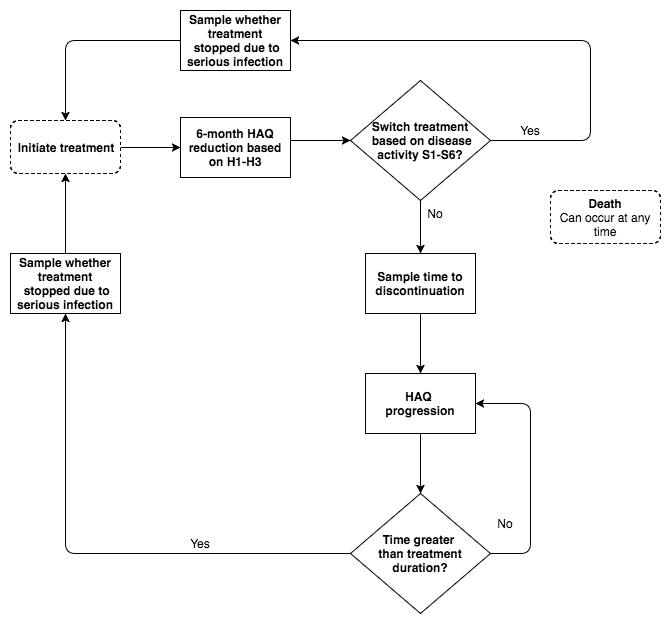
\includegraphics[max size={\textwidth}{\textheight}]{flow-diagram.png}
\caption{Flow diagram of the simulation for a single
patient}\label{fig:flow-diagram}
\begin{minipage}{\linewidth}
\footnotesize
Notes: Rectangles represent ``processes'' determining the effect of treatment on disease progression, Diamonds represent ``decisions'' that determine whether a patient will switch to a new treatment. Dotted lines denote start of a new treatment or the end of the simulation. 
\end{minipage}
\end{figure}

The influence diagram in \autoref{fig:influence-diagram} summarizes the assumed relationships among different variables in the model. Each arrow represents the direct effect of one parameter on another. Dashed lines represent relationships that depend on the structural assumptions used. \autoref{subfig:treatment-effects} focuses on the effect of treatment on disease progression and adverse events while \autoref{subfig:model-outcomes} looks at the variables influencing the primary health and cost outcomes. 

Model outcomes depend on patient characteristics, which have a direct effect on HAQ progression, mortality, and utility. The primary health outcome is the QALY, which depends on mortality and utility. Total costs consist of health care sector costs and productivity losses. The components of health sector costs include drug acquisition and administration costs, general management and monitoring costs, adverse event costs, and hospitalization costs. Analyses from a societal perspective would include productivity losses while analyses from a health care sector perspective would not. The value of treatment is estimated using the net-monetary benefit (NMB), which is calculated by multiplying QALYs by a willingness to pay threshold and subtracting costs ($NMB = QALYs \cdot WTP - Costs$). 

\begin{figure}
\centering
\begin{subfigure}{\textwidth}
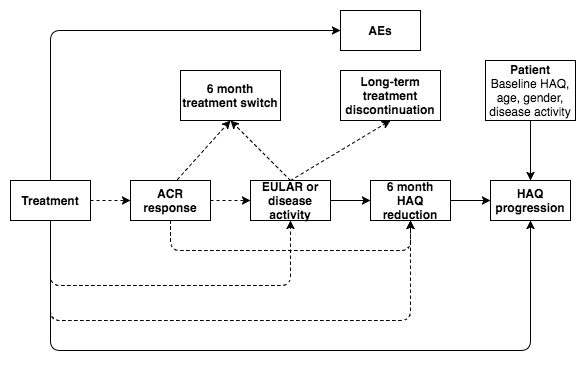
\includegraphics[width=\textwidth]{influence-diagram-a.png}
\caption{Treatment effects} \label{subfig:treatment-effects}
\end{subfigure}
\begin{subfigure}{\textwidth}
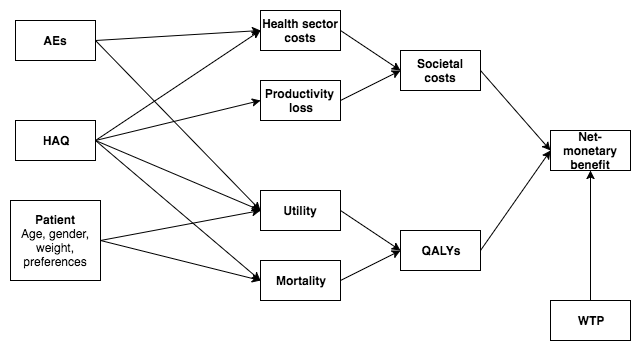
\includegraphics[width=\textwidth]{influence-diagram-b.png}
\caption{Model outcomes} \label{subfig:model-outcomes}
\end{subfigure}
\caption{Influence diagram outlining structural relationships}\label{fig:influence-diagram}
\begin{minipage}{\linewidth}
\footnotesize
Notes: ACR: American College of Rheumatology; EULAR: European League Against Rheumatism; HAQ: Health Assessment Questionnaire: AEs: adverse events; QALYs: quality-adjusted life-years; WTP: willingness to pay. Disease activity refers to the Disease Activity Score with 28-joint counts (DAS28), the Simplified Disease Activity Index (SDAI), or the Clinical Disease Activity Index (CDAI).
\end{minipage}
\end{figure}

\section{Populations}\label{sec:populations}
To run the IPS, a patient population must be specified. The model is designed for patients who are cDMARD experienced. The patient characteristics that must be included in the analysis are age, HAQ, gender, weight, the number of previous DMARDs, and disease activity. These variables are measured at the start of the simulation (i.e., model cycle 0).  

Two default options for the patient population are available. First, a homogeneous cohort of men and women with gender-specific weights but otherwise identical characteristics can be used. Second, a heterogeneous cohort of patients with gender-specific weights but varying across all other characteristics can be specified. Other populations (i.e., for certain subgroups or based on registry data) can be used as well but are not prespecified in our \R{} package. 



Our default population consists of individuals that, on average, have high disease activity. The proportion that is female, age, the number of previous DMARDs, baseline HAQ, and DAS28 are based on the values reported in \citet{curtis2010comparison}. Mean values for the SDAI and CDAI are from the US301 clinical trial---which had a DAS28 score similar to the value from \citet{curtis2010comparison}---summarized in \citet{smolen2003simplified}. Summaries of each variable are reported in \autoref{tbl:pats}. Details on the algorithm for simulating heterogeneous patients are described in \autoref{app:population}.

\begin{table}[!ht]
\begin{center}
\begin{threeparttable}
\caption{Default patient population} \label{tbl:pats}
\begin{tabularx}{\textwidth}{@{\extracolsep{\fill}}lcccc}
\hline
\multicolumn{1}{l}{} & \multicolumn{1}{c}{Mean} & \multicolumn{1}{c}{Standard deviation} & \multicolumn{1}{c}{Minimum} & \multicolumn{1}{c}{Maximum}\\
\hline
\ExpandableInput{tables/pat-inputs.txt}
\hline
\end{tabularx}
\scriptsize
\end{threeparttable}
\end{center}
\end{table}

\section{Source data and parameter estimation}\label{sec:data-parameters}

\subsection{Comparative treatment efficacy from NMA}\label{nma-parameters}
The effect of treatment on ACR response, DAS28, and HAQ at 6 months for bDMARD naive patients are estimated using Bayesian network meta-analyses (NMA) of published randomized controlled trials (RCTs). Primary outcomes were ACR response, change in DAS28 from baseline at 6 months, and the change in HAQ from baseline at 6 months. Results from the NMA are shown in \autoref{tbl:nma-acr-das28-haq}. Details of the systematic literature review and the statistical methodology are provided in the Appendix (\autoref{app:nma-statistical-models}).



\begin{sidewaystable}
\begin{center}
\begin{threeparttable}
\caption{NMA estimates of ACR response, change in DAS28, and change in HAQ for biologic naive patients} \label{tbl:nma-acr-das28-haq}
\small
\begin{tabular}{lccccc}
\hline
\multicolumn{1}{c}{} & \multicolumn{3}{c}{ACR response} & \multicolumn{2}{c}{}\\
\cmidrule(lr){2-4} 
\multicolumn{1}{l}{} & \multicolumn{1}{c}{ACR20} & \multicolumn{1}{c}{ACR50} & \multicolumn{1}{c}{ACR70} & \multicolumn{1}{c}{$\Delta$DAS28} & \multicolumn{1}{c}{$\Delta$HAQ} \\
\hline
\ExpandableInput{tables/nma-acr-das28-haq.txt}
\hline
\end{tabular}
\scriptsize
Notes: ACR20/50/70 categories are the probability of at least a 20/50/70\% improvement. 95\% credible intervals are in parentheses. Estimates are based on 1,000 random draws of the NMA parameters. $\Delta$DAS28 and $\Delta$HAQ are changes in the DAS28 and HAQ score from their baseline scores respectively; negative numbers denote reductions in baseline values. cDMARDs = conventional disease-modifying antirheumatic drugs; MTX = methotrexate; ABT IV = abatacept intravenous; ADA = adalimumab; ETN = etanercept; GOL = golimumab; IFX = infliximab; TCZ = tocilizumab; CZP = certolizumab pegol; ABT SC = abatacept subcutaneous; RTX = rituximab; TOF = tofacitinib. ACR = American College of Rheumatology.
\end{threeparttable}
\end{center}
\end{sidewaystable}


Treatment effects for bDMARD experienced patients were reduced by applying the relative risk ratio reported in \citet{carlson2015economic}. More specifically, reductions in DAS28 and HAQ scores for bDMARD experienced patients are assumed to be, on average, 84\% of the reduction in DAS28 and HAQ scores for bDMARD naive patients. Likewise, we assume that the mean reduction in overlapping ACR response categories (ACR 20/50/70) is 84\% after failing the first bDMARD, implying that an ACR response of 60/40/20 would, on average, be reduced to 50/33/16. To capture uncertainty, the reduction in treatment effects is assumed to be distributed uniformly with lower and upper bounds of 74\% and 94\% respectively. 

In the simulation, treatment efficacy depends on the line of therapy and whether a patient is bDMARD naive or bDMARD experienced at baseline. For bDMARD naive patients, first line treatment response is based on the NMA results for bDMARD naive patients while efficacy for all other treatments in a treatment sequence are reduced using the relative risk ratio. For bDMARD experienced patients, treatment response is reduced using the relative risk ratio at each line of therapy including the first line. 

\subsection{Treatment switching at 6 months}
The data required to determine treatment switching at 6 months depends on the selected model structure. If \textbf{S1} is selected, then treatment switching depends on the simulated ACR response; likewise, if \textbf{S5} is selected, then treatment switching depends on the simulated level of DAS28 at 6 months. When \textbf{S2-S4} are used, treatment switching is determined by the relationship between ACR response and the change in disease activity, and in \textbf{S6}, switching is based on the relationship between ACR response and EULAR response. Details of the mapping between ACR response and change in disease activity and between ACR response and EULAR response are provided below.  

\subsubsection{ACR response and change in disease activity}
There are currently no established mappings between mutually exclusive ACR response categories and DAS28, SDAI, or CDAI \citep{madan2015consensus}. However, \citet{aletaha2005simplified} provides evidence on the relationship between overlapping ACR response categories (ACR 20/50/70) and mean changes in each of the three disease activity measures. Results are reported for three cohorts---the Leflunomide datasets, the inception cohort, and the routine cohort---with 1,839, 91, and 279 patients, respectively. We transformed mean changes by overlapping ACR response categories to mean changes by mutually exclusive ACR response categories by using the number of patients in each mutually exclusive ACR response category as described in \autoref{app-acr-da}. \citet{smolen2003simplified} provided the number of patients in each ACR response category in the Leflunomide dataset and \citet{aletaha2005acute} provided the number of patients in the inception cohort. Mean changes in disease activity in each mutually exclusive ACR response category are shown in \autoref{tbl:acr2da}.



\begin{table}[!ht]
\begin{center}
\begin{threeparttable}
\caption{Relationship between ACR response and change in disease activity measures} \label{tbl:acr2da}
\begin{tabularx}{\textwidth}{@{\extracolsep{\fill}}lcccc}
\hline
\multicolumn{1}{l}{ACR response} &  \multicolumn{3}{c}{Mean change at 6 months}\\
\cmidrule{2-5}
\multicolumn{1}{l}{} & \multicolumn{1}{c}{Leflunomide dataset} & \multicolumn{3}{c}{Inception cohort}\\
\cmidrule(lr){2-2}  \cmidrule(lr){3-5}
\multicolumn{1}{c}{} & \multicolumn{1}{c}{SDAI} & \multicolumn{1}{c}{SDAI} &\multicolumn{1}{c}{CDAI} & \multicolumn{1}{c}{DAS28} \\
\hline
\ExpandableInput{tables/acr2da.txt}
\hline
\end{tabularx}
\scriptsize
\end{threeparttable}
\end{center}
\end{table}

We did not include estimates from the routine cohort for two reasons. First, we were unable to find information on the number of patients in each ACR response category. Second, patients in the routine cohort had considerably lower disease activity levels \citep{aletaha2005simplified, aletaha2005acute} and our default population (see \autoref{sec:populations}) consists of patients with high disease activity at baseline. Mean DAS28 in the inception cohort and routine cohort were 5.62 and 4.09, respectively, while the mean DAS 28 ranged from 6.3 to 7 across the clinical trials making up the Leflunomide dataset.

\subsubsection{ACR response and change in EULAR response}
ACR responses were translated into EULAR response probabilities based on evidence of their relationship reported in \citet{stevenson2016adalimumab} and obtained from the US Veterans Affairs Rheumatoid Arthritis (VARA) registry (\autoref{tbl:acr2eular}).




\begin{table}[!ht]
\begin{center}
\begin{threeparttable}
\caption{Relationship between ACR response and EULAR response} \label{tbl:acr2eular}
\begin{tabularx}{\textwidth}{@{\extracolsep{\fill}}lcccc}
\hline
\multicolumn{1}{l}{} & \multicolumn{3}{c}{EULAR response} \\
\cmidrule{2-4} 
\multicolumn{1}{c}{ACR response} & \multicolumn{1}{c}{None} & \multicolumn{1}{c}{Moderate} & \multicolumn{1}{c}{Good} \\
\hline
\ExpandableInput{tables/acr2eular.txt}
\hline
\end{tabularx}
\scriptsize
Notes: The VARA registry is a multicentre, US database of veterans age 19 and older. Each cell represents the number of patients in the 
database in a given category. 
\end{threeparttable}
\end{center}
\end{table}

\subsection{Change in HAQ at 6 months}
As in \citet{icer2017tim}, ACR responses from the NMA were translated into HAQ scores based on evidence from the adalimumab monotherapy for treatment of rheumatoid arthritis (ADACTA) trial reported in \citet{carlson2015economic} (\autoref{tbl:acr2haq}).



\begin{table}[!ht]
\begin{center}
\begin{threeparttable}
\caption{Relationship between ACR response and change in HAQ at 6 months} \label{tbl:acr2haq}
\begin{tabularx}{\textwidth}{@{\extracolsep{\fill}}lcc}
\hline
\multicolumn{1}{l}{} & \multicolumn{2}{c}{HAQ change} \\
\cmidrule{2-3} 
\multicolumn{1}{c}{ACR response} & \multicolumn{1}{c}{Mean} & \multicolumn{1}{c}{Standard error} \\
\hline
\ExpandableInput{tables/acr2haq.txt}
\hline
\end{tabularx}
\scriptsize
Source: \citet{carlson2015economic}
\end{threeparttable}
\end{center}
\end{table}



The relationship between EULAR response and HAQ is based on analyses conducted by \citet{stevenson2016adalimumab} using the BSRBR database. Their analysis is based on predictions from a mixture model with covariates set to sample means. Moderate and good EULAR responses are associated with -0.317 (SE = 0.048) and -0.672 (SE = 0.112) changes in HAQ scores respectively (\autoref{tbl:eular2haq}). 

\begin{table}[!ht]
\begin{center}
\begin{threeparttable}
\caption{Relationship between EULAR response and HAQ} \label{tbl:eular2haq}
\begin{tabularx}{\textwidth}{@{\extracolsep{\fill}}lcc}
\hline
\multicolumn{1}{c}{EULAR response} & \multicolumn{1}{c}{Mean} & \multicolumn{1}{c}{SE} \\
\hline
\ExpandableInput{tables/eular2haq.txt}
\hline
\end{tabularx}
\scriptsize
%Notes: 
\end{threeparttable}
\end{center}
\end{table}

\autoref{tbl:sim-haq-change} compares the impact of treatment on HAQ using model structures \textbf{H1-H3}. There is considerable variation, which suggests that the choice of model structure has important consequences for cost-effectiveness. The effect of treatment on the change in HAQ is largest when modeled directly (\textbf{H2}) and smallest when modeled through both ACR and EULAR response (\textbf{H3}). 95\% credible intervals are also considerably larger when the change in HAQ is modeled indirectly (\textbf{H1} and \textbf{H3}), then when it is modeled directly (\textbf{H2}). 





\begin{table}[!ht]
\begin{center}
\begin{threeparttable}
\caption{Simulated change in HAQ at 6 months under different model structures} \label{tbl:sim-haq-change}
\begin{tabularx}{\textwidth}{@{\extracolsep{\fill}}lccc}
\hline
\multicolumn{1}{l}{} & \multicolumn{1}{c}{\textbf{H1}} & \multicolumn{1}{c}{\textbf{H2}} & \multicolumn{1}{c}{\textbf{H3}} \\
\hline
\ExpandableInput{tables/sim-dhaq-6months.txt}
\hline
\end{tabularx}
\scriptsize
Notes: \textbf{H1}, \textbf{H2}, and \textbf{H3} are the Treatment $\rightarrow$ ACR $\rightarrow$ HAQ, Treatment $\rightarrow$ HAQ, and Treatment $\rightarrow$ ACR $\rightarrow$ EULAR $\rightarrow$ HAQ pathways respectively. 95\% credible intervals are in parentheses. Estimates are based on 6-month simulations of 1,000 patients and 1,000 parameters sets for each therapy. $\Delta$HAQ denotes a change in the HAQ score at 6 months from baseline; a negative value indicates a reduction in the HAQ score. cDMARDs = conventional disease-modifying antirheumatic drugs; MTX = methotrexate; ABT IV = abatacept intravenous; ADA = adalimumab; ETN = etanercept; GOL = golimumab; IFX = infliximab; TCZ = tocilizumab; CZP = certolizumab pegol; ABT SC = abatacept subcutaneous; RTX = rituximab; TOF = tofacitinib. ACR = American College of Rheumatology.
\end{threeparttable}
\end{center}
\end{table}

\subsection{HAQ progression in the absence of bDMARD treatment}\label{haq-progression-in-the-absence-of-bdmard-treatment}

The natural course of HAQ progression in the absence of bDMARDs develops over time according to an estimated natural course for patients remaining on cDMARDs or following discontinuation of the last bDMARD of the sequence (i.e., on NBT). The natural course of HAQ can either be assumed to change at a constant linear rate or be modeled using a LCGM that accounts for non-linear progression and heterogeneity across patients. 

\subsubsection{Constant linear rate of progression} \label{sec:haq-linear-rate}
The rate of progression in the linear case is based on the observational study by \citet{wolfe2010loss}. They assessed the development of HAQ over time at six month intervals for up to 11 years among 3,829 RA patients who switched from non-biologic treatment to biologic treatment and participated in the National Data Bank for Rheumatic Diseases (NDB) longitudinal study of RA outcomes. The annual HAQ progression rate prior to biologic therapy was 0.031 (95\% confidence interval (95\%CI): 0.026 to 0.036) and is assumed to reflect the course of progression of HAQ in the absence of bDMARDs.

Based on the same data, \citet{michaud2011treatment} reported overall and age-specific specific HAQ progression rates. The differences between the overall and age specific rates are as follows: \textless{}40: -0.020 (95\%CI: -0.0223 to -0.0177); 40-64: -0.008 (95\%CI: -0.0101 to -0.0059); \(\geq\) 65 0.017 (95\%CI: 0.0136 to 0.0204). These estimates are applied to the overall progression rate of 0.031 to obtain age specific HAQ progression rates (see \autoref{app:age-linear-haq}).



\begin{table}[!ht]
\begin{center}
\begin{threeparttable}
\caption{Annual linear progression of HAQ in the absence of bDMARDs beyond 6 months} \label{tbl:haq-lprog}
\footnotesize
\begin{tabularx}{\textwidth}{@{\extracolsep{\fill}}lrrrl}
\hline
\multicolumn{2}{l}{} & \multicolumn{2}{c}{95\% CI} & \multicolumn{1}{l}{} \\
\cmidrule{3-4} 
\multicolumn{1}{l}{} & \multicolumn{1}{r}{Estimate} & \multicolumn{1}{r}{Lower} & \multicolumn{1}{r}{Upper} & \multicolumn{1}{l}{Reference} \\
\hline
Overall progression rate \\
\ExpandableInput{tables/haq-lprog-cdmards.txt}
Change in overall progression rate by age \\
\ExpandableInput{tables/haq-lprog-diff-byage.txt}
\hline
\end{tabularx}
\scriptsize
Notes: 95\% confidence intervals are calculated using a normal distribution. Confidence intervals for changes in HAQ progression rates by age assume no covariance between the overall progression rate and the age-specific rates reported by \citet{michaud2011treatment}.
\end{threeparttable}
\end{center}
\end{table}

\subsubsection{Latent class growth model} \label{sec:haq-lcgm}
We also model the rate of HAQ progression in the absence of bDMARDs using a mixture model approach that has increasingly been used to model HAQ progression over time \citep{stevenson2016adalimumab, norton2013trajectories, norton2014health}. These models suggest that different subgroups have distinct HAQ trajectories and that the rate of worsening of HAQ progression decreases over time. We use the LCGM estimated by \citet{norton2014health} and since we aim to model trajectories for cDMARDs and NBTs we chose the specification based on data from the Early Rheumatoid Arthritis Cohort Study (ERAS) cohort, which has a high percentage of patients receiving methotrexate and a very small percentage receiving biologics. Complete details of the LCGM are provided in \autoref{app:lcgm-haq}. 



The \citet{norton2014health} LCGM determined that there are four classes of patients and thus four distinct HAQ trajectories. The probability of class membership depends on 7 variables: age, gender, DAS28, disease duration, rheumatoid factor, the ACR 1987 criteria for RA, and a measure of socioeconomic status. Age, gender, and the DAS28 are relevant to the way the population is defined within our model (see \autoref{sec:populations}) and are therefore important determinants of the HAQ trajectory. Other variables (disease duration, rheumatoid factor, ACR criteria, and socioeconomic status) are not defined within our population. We consequently set disease duration (8.2 months), rheumatoid factor (0.73), and the socioeconomic status variable (0.49) equal to their mean values with the ERAS cohort. The ACR criteria was set to 1. 

HAQ trajectories (in levels) by class are shown \autoref{fig:lcgm-haq-prog}. The dotted lines plot observed mean values. There are clear distinguishable classes as both the level of the HAQ score and its slope vary between groups. \citet{norton2014health} refer to the groups as ``low'', ``moderate'', ``high'', and ``severe'' groups, in order from the lowest to highest HAQ scores. The observed trends for the low, medium, and high groups follow a J-shaped pattern with a sharp drop following treatment initiation and an upward slope thereafter, while the severe group experiences persistently high HAQ scores. Since our model separates the initial treatment phase from the maintenance phase, we are only concerned with HAQ progression following the initial drop. As in \citet{stevenson2016adalimumab}, we consequently only predict values from year 2 onward. The fitted values are the solid upward sloping lines in the plot.  
\begin{figure}[H]
\centering
\includegraphics[max size={.8\textwidth}{.8\textheight}]{../../data-raw/figs/haq-lcgm-obsexp.pdf}
\caption{Observed and predicted HAQ trajectories in the ERAS dataset from the latent class growth model}\label{fig:lcgm-haq-prog}
\begin{minipage}{\linewidth}
\footnotesize
Notes: The first three data points corresponds to years 0, 0.5, and 1, respectively; all other data points are spaced 1 year apart.
\end{minipage}
\end{figure}



An important question for cost-effectiveness modeling in RA is how the rate of progression within each class in the LCGM compares to a constant linear trajectory. We examine this question in \autoref{fig:lcgm-vs-linear}, which compares yearly rates of changes in HAQ using the LCGM and with constant annual rates of change (0.031 per year) based on the \citet{wolfe2010loss} analysis. The LCGM was simulated over 30 years and differences between year $t$ and year $t-1$ were used to assess changes in HAQ score from one year to the next.  

In the moderate, high, and severe groups the rate of HAQ progression is higher initially in the LCGM than in the \citet{wolfe2010loss} analysis; however, the LCGM modeled rate of HAQ progression declines over time and eventually begins to approach zero. In the low group, HAQ increases at a rate less than 0.031 per year and the rate of increase declines over time. 

\begin{figure}[H]
\centering
\includegraphics[max size={.7\textwidth}{.7\textheight}]{figs/haq-lcgm-vs-linear.png}
\caption{A comparison of predicted yearly changes in HAQ between a latent class growth model and constant linear progression from year 2 onwards}\label{fig:lcgm-vs-linear}
\end{figure}

\subsection{HAQ trajectory with bDMARD maintenance treatment}
Based on the NDB longitudinal study, \citet{wolfe2010loss} estimated the overall annual HAQ progression rate among RA patients who had switched to biologic treatment at -0.001 (95CI: -0.004 to 0.002). In a separate analysis, also based on NDB data, \citet{michaud2011treatment} reported annual HAQ progression rates by treatment adjusted for baseline HAQ score, age, sex, education, smoking, BMI, comorbidity, and RA onset. The average HAQ rate among patients on a biologic was -0.001 as well, which instills confidence that the reported HAQ progression rates for different bDMARDs as reported by \citet{michaud2011treatment} can be directly compared with the overall annual HAQ progression rate of 0.031 reported by \citet{wolfe2010loss}. Accordingly, bDMARD specific HAQ progression rates by \citet{michaud2011treatment} are used in the model. For bDMARD treatments evaluated in the model for which no HAQ progression rate was reported by \citet{michaud2011treatment}, the overall biologic rate of -0.001 is used. 

\subsection{Duration of maintenance treatment}\label{duration-of-maintenance-treatment}
Time to treatment discontinuation in the maintenance phase depends on the pathway (\textbf{S1-S6}) used to model treatment switching. If \textbf{S1} is selected, a single treatment discontinuation curve based on an analysis from the CORRONA database is used for all patients. In \textbf{S2-S5}, time to treatment discontinuation is stratified by the level of disease activity, and in \textbf{S6} treatment duration depends on EULAR response.  

\subsubsection{Treatment duration in the US}\label{sec:ttd-overall}
We based our estimates of treatment duration during the maintenance phase for patients in the US with analyses of the CORRONA database \citep{strand2013op0064}. The analysis sample consisted of 6,209 patients age 18 or older treated between 2002 and 2011 receiving either TNF inhibitors or other bDMARDs. The mean age was 57.6 years, 43\% of patients were biologic naive, the mean CDAI was 16, and just over 26\% of patients had high disease activity (CDAI $\geq$ 22). 

7 parametric survival models (exponential, Weibull, Gompertz, gamma, log-logistic, lognormal, and generalized gamma) were estimated on individual patient data reconstructed from a Kaplan-Meier curve from the CORRONA analysis using the algorithm developed in \citet{guyot2012enhanced}. We compared fit using the Akaike Information Criteria (AIC) and Bayesian Information Criteria (BIC). The generalized gamma had the lowest AIC and BIC, so we consider it to be the preferred model. A plot of of the generalized gamma distribution against the Kaplan-Meier curve is shown in \autoref{fig:corrona-gg}. As can be seen in the plot, the shape of the survival curve estimated using a generalized gamma distribution tracks the Kaplan-Meier curve closely.  



\begin{table}[!ht]
\begin{center}
\begin{threeparttable}
\caption{AIC and BIC for parametric models of treatment duration from the CORRONA database} \label{tbl:ic-ttd-corrona}
\begin{tabularx}{\textwidth}{@{\extracolsep{\fill}}lcccc}
\hline
\multicolumn{1}{l}{Distribution} & \multicolumn{1}{c}{AIC} & \multicolumn{1}{c}{BIC}  \\
\hline
\ExpandableInput{tables/ttd-corrona-ipdsurv-ic.txt}
\hline
\end{tabularx}
\end{threeparttable}
\end{center}
\end{table}

\begin{figure}[h]
\centering
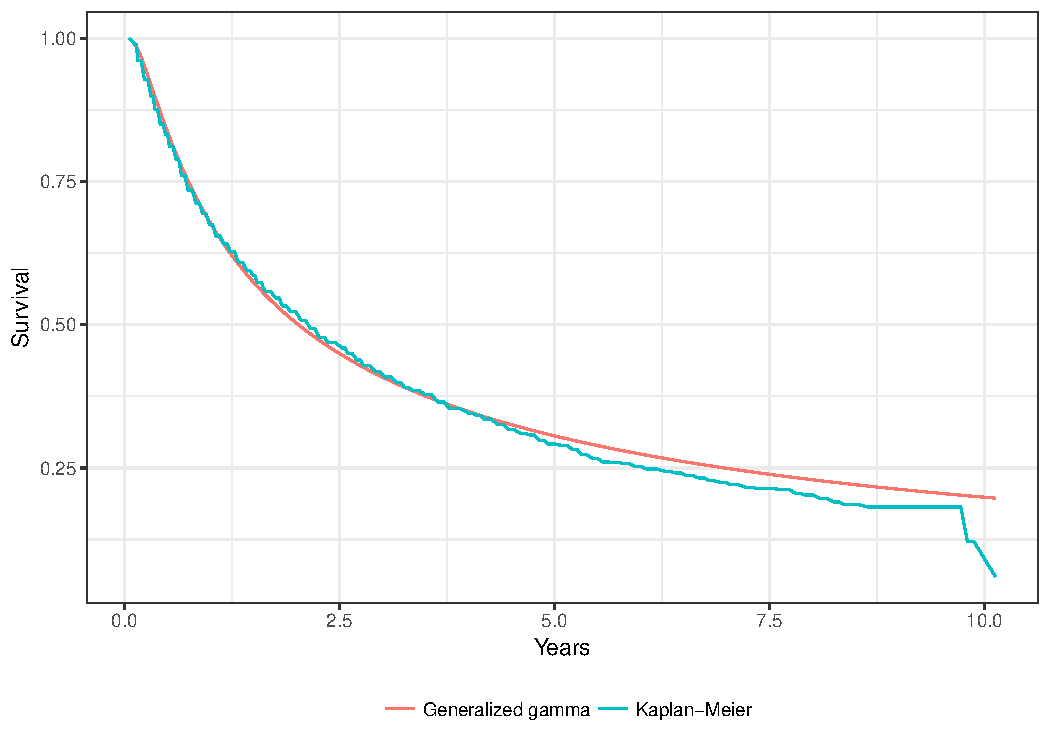
\includegraphics[max size={.7\textwidth}{.7\textheight}]{../../data-raw/figs/ttd-corrona-ipdsurv-gengamma.pdf}
\caption{Generalized gamma and Kaplan-Meier time to treatment discontinuation curves using reconstructed individual patient data from the CORRONA database}\label{fig:corrona-gg}
\end{figure}

We considered estimating separate time to discontinuation curves for each therapy, but did not for a number of the reasons cited in \citet{stevenson2016adalimumab}. The majority of the literature focuses on anti-TNFs (e.g., infliximab, etanercept, and adalimumab) \citep[e.g.][]{gomez2006switching, yazici2009changing, pan2009comparison}, which makes it difficult to estimate discontinuation curves for the other therapies. Furthermore, studies comparing rates of discontinuation across therapies tend to be observational because clinical trials are of short duration and do not reflect real-world patient populations. However, although observational studies provide accurate predictions on time to discontinuation, it is difficult to avoid bias from confounding when estimating differences across treatments because patients are not randomized into treatment and control groups \citep{souto2015rate} .   

We also lack data on treatment duration for patients on cDMARDs. Following \citet{stevenson2016adalimumab}, we assume that, conditional on continuing treatment at 6 months, treatment duration for bDMARDs is applicable to treatment duration for cDMARDs. This is, in turn, based on the assumption that cDMARDs are not likely to be more toxic than biologics used in combination with cDMARDs. 

\subsubsection{Treatment duration by disease activity level}\label{ttd-da}
When \textbf{S2-S5} are selected, treatment duration is stratified by the level of disease activity. Since patients in the CORRONA database tended to have moderate disease activity (mean CDAI = 16), we use the CORRONA survival curve to model treatment duration for patients with moderate disease activity. We adjust this curve for patients in remission or low disease activity using the odds ratios reported in \citet{zhang2011thresholds}, which imply that patients in remission or with low disease activity have .52 times the odds of stopping treatment as patients with moderate disease activity. In particular, we adjust the probability of treatment failure at each point in time using the methodology described in \autoref{app:odds-ratio-prob}. As with the analysis described in \autoref{sec:ttd-overall}, we then fit 7 parametric survival models to individual patient data reconstructed from the adjusted survival curve using the \citet{guyot2012enhanced} algorithm. Generalized gamma time to treatment discontinuation curves stratified by disease activity level are shown in \autoref{fig:ttd-gg-da}.

\begin{figure}[H]
\centering
\includegraphics[max size={.7\textwidth}{.7\textheight}]{../../data-raw/figs/ttd-corrona-ipdsurv-gengamma-by-da.pdf}
\caption{Generalized gamma time to treatment discontinuation curves by disease activity level}\label{fig:ttd-gg-da}
\end{figure}

\subsubsection{Treatment duration by EULAR response} \label{ttd-eular}
In \textbf{S6}, we stratify time to treatment discontinuation by EULAR response based on analyses of the British Society for Rheumatology Biologics Registers (BSRBR) database \citep{stevenson2016adalimumab}. We again fit 7 parametric survival models using reconstructed individual patient data. The survival curves reported in \citet{stevenson2016adalimumab} were used to create the patient data. The AIC and BIC of each model by EULAR response category are shown in \autoref{tbl:ic-dur-eular}.



\begin{table}[!ht]
\begin{center}
\begin{threeparttable}
\caption{AIC and BIC for parametric models of treatment duration by EULAR response} \label{tbl:ic-dur-eular}
\begin{tabularx}{\textwidth}{@{\extracolsep{\fill}}lcccc}
\hline
\multicolumn{1}{l}{} & \multicolumn{2}{c}{Moderate EULAR response} & \multicolumn{2}{c}{Good EULAR response} \\
\cmidrule{2-3} \cmidrule{4-5}
\multicolumn{1}{l}{Distribution} & \multicolumn{1}{c}{AIC} & \multicolumn{1}{c}{BIC} & \multicolumn{1}{c}{AIC}  & \multicolumn{1}{c}{BIC}   \\
\hline
\ExpandableInput{tables/ttd-bsrbr-ipdsurv-eular-ic.txt}
\hline
\end{tabularx}
\end{threeparttable}
\end{center}
\end{table}

One concern is that the BSRBR is representative of the UK but not the US. As a result, we also estimate ``adjusted'' survival models appropriate for US based analyses. The adjustment is made in six steps using the analyses from the CORRONA database described in \autoref{sec:ttd-overall}. 

\begin{enumerate}
\def\labelenumi{\arabic{enumi}.}
\item Calculate a hazard function based on a survival curve from an analysis
  of the CORRONA database. In particular, reconstruct individual patient
  data from the survival curve \citep{guyot2012enhanced} and fit a
  spline-based survival model. Then use the spline-based model to
  estimate the hazard function $h(t)_{corrona}$.
\item Calculate a hazard function based on the BSRBR. To do so, first
  calculate hazard functions for both moderate and good EULAR responders
  using the same method described in step 1. Then calculate an overall
  hazard function with the proportion of moderate and good responders in
  the BSRBR analysis. Given that the number of moderate responders is
  \(5,492\) and the number of good responders is $2,417$ the overall
  hazard function is $h(t)_{bsrbr} = \frac{5,492}{7,909}h(t)_{bsrbr, moderate} + \frac{2,417}{7,909}h(t)_{bbsrbr, good}$.
\item At each point in time, calculate the ratio of the CORRONA and BSRBR
  hazard functions: $HR(t) = h(t)_{corrona}/h(t)_{bbsrbr}$.
\item Apply the hazard ratio in step 3 to the BSRBR hazard functions for
  each EULAR response category. That is $h(t)_{bsrbr, moderate, adj} = h(t)_{bsrbr, moderate} \cdot HR(t)$ and $h(t)_{bsrbr, good, adj} = h(t)_{bsrbr, good} \cdot HR(t)$.
\item Generate survival curves using the hazard functions from step 4.
  Specifically, given a general hazard function $h(t)$, calculate the
  cumulative hazard function, $H(t) = \int_{z = 0}^{t} h(z)dz$,
  convert this to a survival function using $S(t) = exp(-H(t))$, and
  reconstruct individual patient data using the survival curve.
\item Fit parametric survival models to the individual patient data
  generated in step 5.
\end{enumerate}

Both adjusted and unadjusted survival curves by EULAR response fit using a generalized gamma distribution are shown in \autoref{fig:bsrbr-gg}. AIC and BIC for the parametric models fit in step 6 to the adjusted individual patient data are shown in \autoref{tbl:ic-dur-adj-eular}.

\begin{figure}[h]
\centering
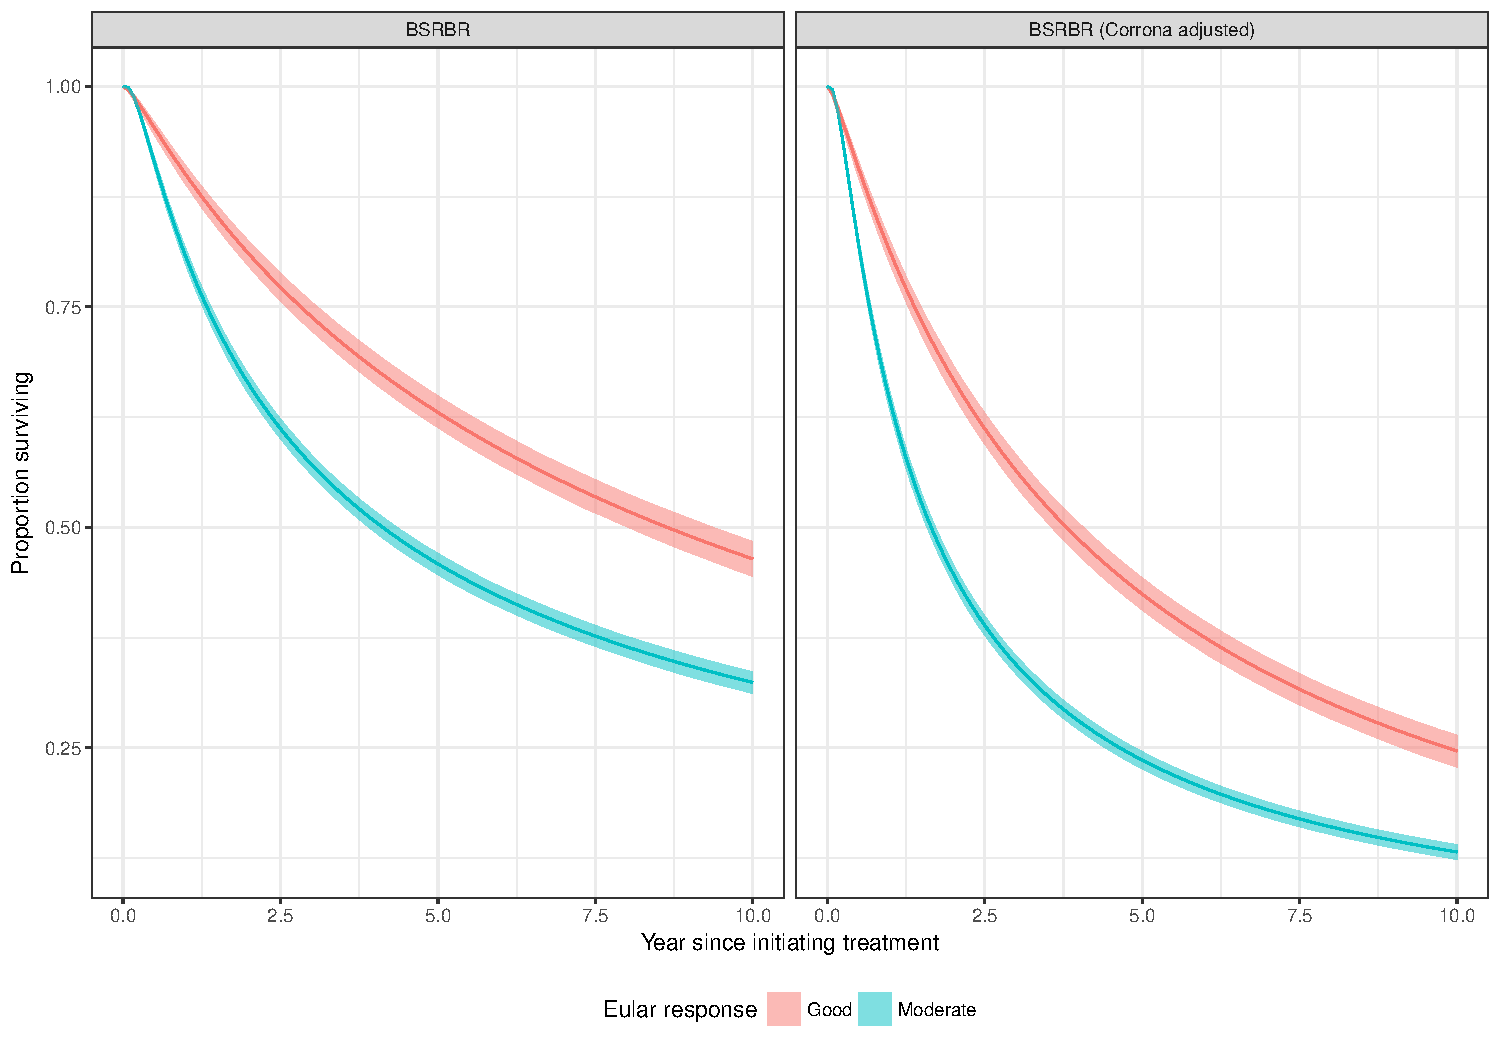
\includegraphics[max size={.7\textwidth}{.7\textheight}]{../../data-raw/figs/ttd-bsrbr-ipdsurv-comp-gengamma-by-eular.pdf}
\caption{Generalized gamma survival curve of treatment duration using reconstructed individual patient data based on analyses from Stevenson et al. (2016) by EULAR response category}\label{fig:bsrbr-gg}
\end{figure}




\begin{table}[!ht]
\begin{center}
\begin{threeparttable}
\caption{AIC and BIC for CORRONA adjusted parametric models of treatment duration by EULAR response} \label{tbl:ic-dur-adj-eular}
\begin{tabularx}{\textwidth}{@{\extracolsep{\fill}}lcccc}
\hline
\multicolumn{1}{l}{} & \multicolumn{2}{c}{Moderate EULAR response} & \multicolumn{2}{c}{Good EULAR response} \\
\cmidrule{2-3} \cmidrule{4-5}
\multicolumn{1}{l}{Distribution} & \multicolumn{1}{c}{AIC} & \multicolumn{1}{c}{BIC} & \multicolumn{1}{c}{AIC}  & \multicolumn{1}{c}{BIC}   \\
\hline
\ExpandableInput{tables/ttd-bsrbr-ipdsurv-eular-adjusted-ic.txt}
\hline
\end{tabularx}
\end{threeparttable}
\end{center}
\end{table}

\FloatBarrier


\subsection{Rebound post treatment}
Since no data exists on the size of the HAQ rebound post treatment, we vary its size as a proportion of the initial 6-month HAQ decline. 1 is used as an upper bound, which implies that the HAQ rebound is equal to the improvement experienced at the end of the initial 6-month period with that treatment. 0.7 is currently used as a lower bound.

\subsection{Serious infections}
Based on the NMA by \citet{singh2011adverse} and in accordance with \citet{stevenson2016adalimumab}, we assume a rate of 0.035 (95\% CI: 0.027 to 0.046) infections per person-year with all bDMARDs and a rate of 0.026 (no CI reported) infections per person-year with cDMARDs. The rate of infection is assumed to be equal across bDMARDs because the published results for specific bDMARDs are estimated with very little precision. The standard error on the infection rate for bDMARDs is assumed to be the same as the standard error for cDMARDs since no standard error was reported for bDMARDs in \citet{singh2011adverse}.



A patient in the IPS has a serious infection if the simulated time to serious infection occurs before the simulated time of treatment discontinuation. \autoref{tbl:si-prob} shows the probability of this occurring when treatment duration is modeled using a generalized gamma distribution. The probability of a serious infection is relatively rare as only 3.48\% of patients using cDMARDs and 8.07\% of patients using bDMARDs have serious infections. However, differences between cDMARDs and bDMARDs are not insignificant as the probability of a serious infection is almost 5 percentage points higher with bDMARDs than with cDMARDs.

\begin{table}[!ht]
\begin{center}
\begin{threeparttable}
\caption{Probability of serious infection} \label{tbl:si-prob}
\begin{tabularx}{\textwidth}{@{\extracolsep{\fill}}lrrr}
\hline
\multicolumn{1}{l}{} & \multicolumn{3}{c}{Probability} \\
\cmidrule{2-4} 
\multicolumn{2}{l}{} & \multicolumn{2}{c}{95\% CI} \\
\cmidrule{3-4} 
\multicolumn{1}{c}{} & \multicolumn{1}{c}{Mean} & \multicolumn{1}{c}{Lower} & \multicolumn{1}{c}{Upper} \\
\hline
\ExpandableInput{tables/si-prop-gengamma.txt}
\hline
\end{tabularx}
\scriptsize
Notes: Probabilities are estimated by simulating 1,000 patients and 1,000 parameter sets. Treatment duration is simulated using a generalized gamma distribution. 
\end{threeparttable}
\end{center}
\end{table}

An important question related to the sensitivity of cost-effectiveness to the model specification is whether the probability of serious infections depends on the distribution used to model time to treatment discontinuation. \autoref{tbl:si-prop-bydist} consequently compares serious infection probabilities by the time to treatment discontinuation distribution. There are very small differences across distributions, suggesting that the treatment duration distribution has almost no impact on the probability of serious infections.  

\begin{table}[!ht]
\begin{center}
\begin{threeparttable}
\caption{Probability of serious infection with cDMARDs by distribution used to model treatment duration} \label{tbl:si-prop-bydist}
\begin{tabularx}{.5\textwidth}{l@{\extracolsep{\fill}}r}
\hline
\multicolumn{1}{c}{Distribution} & \multicolumn{1}{c}{Mean probability} \\
\hline
\ExpandableInput{tables/si-prop-mtx-bydist.txt}
\hline
\end{tabularx}
\scriptsize
Notes: Probabilities are estimated by simulating 1,000 patients and 1,000 parameter sets. 
\end{threeparttable}
\end{center}
\end{table}

\FloatBarrier

\subsection{Utility}\label{utility}
Two algorithms can be used to map HAQ to an EQ-5D utility score. Each is used to simulate utility for every patient in the model to obtain a distribution of utility over time. Our preferred algorithm is the mixture model developed by \citet{alava2013relationship}, which is described in detail in \autoref{app:sim-utility-mixture}. The second algorithm uses the logistic regression equation reported in \citet{wailoo2006modeling}. The regression coefficients from \citet{wailoo2006modeling} are shown in \autoref{tbl:util-wailoo-coef} and are used to predict utility with the inverse logit function.



\begin{table}[!ht]
\begin{center}
\begin{threeparttable}
\caption{Logistic regression coefficient from Wailoo utility algorithm} \label{tbl:util-wailoo-coef}
\begin{tabularx}{\textwidth}{@{\extracolsep{\fill}}lcc}
\hline
\multicolumn{1}{c}{} & \multicolumn{1}{c}{Estimate} & \multicolumn{1}{c}{Standard error}  \\
\hline
\ExpandableInput{tables/util-wailoo-pars.txt}
\hline
\end{tabularx}
\scriptsize
Notes: Coefficients are from the logistic regression reported in \citet{wailoo2006modeling}. 
\end{threeparttable}
\end{center}
\end{table}

\autoref{fig:util-comparison} compares results from the two algorithms. Mean utility scores from the \citet{alava2013relationship} mixture model lie above those from the \citet{wailoo2006modeling} equation for all values of HAQ. Moreover, the slope of utility curve produced from the mixture model is steeper (although less so for the commonly observed HAQ scores between 1 and 1.5), implying that changes in HAQ from the mixture model predict larger changes in utility. Given that the mixture models have been shown to predict utility more accurately \citep{alava2012tails, alava2013relationship, hernandez2014comparison}, this suggests that standard models underestimate the quality-adjusted life-year benefits, and hence, the cost-effectiveness of treatments. 



\begin{figure}
\centering
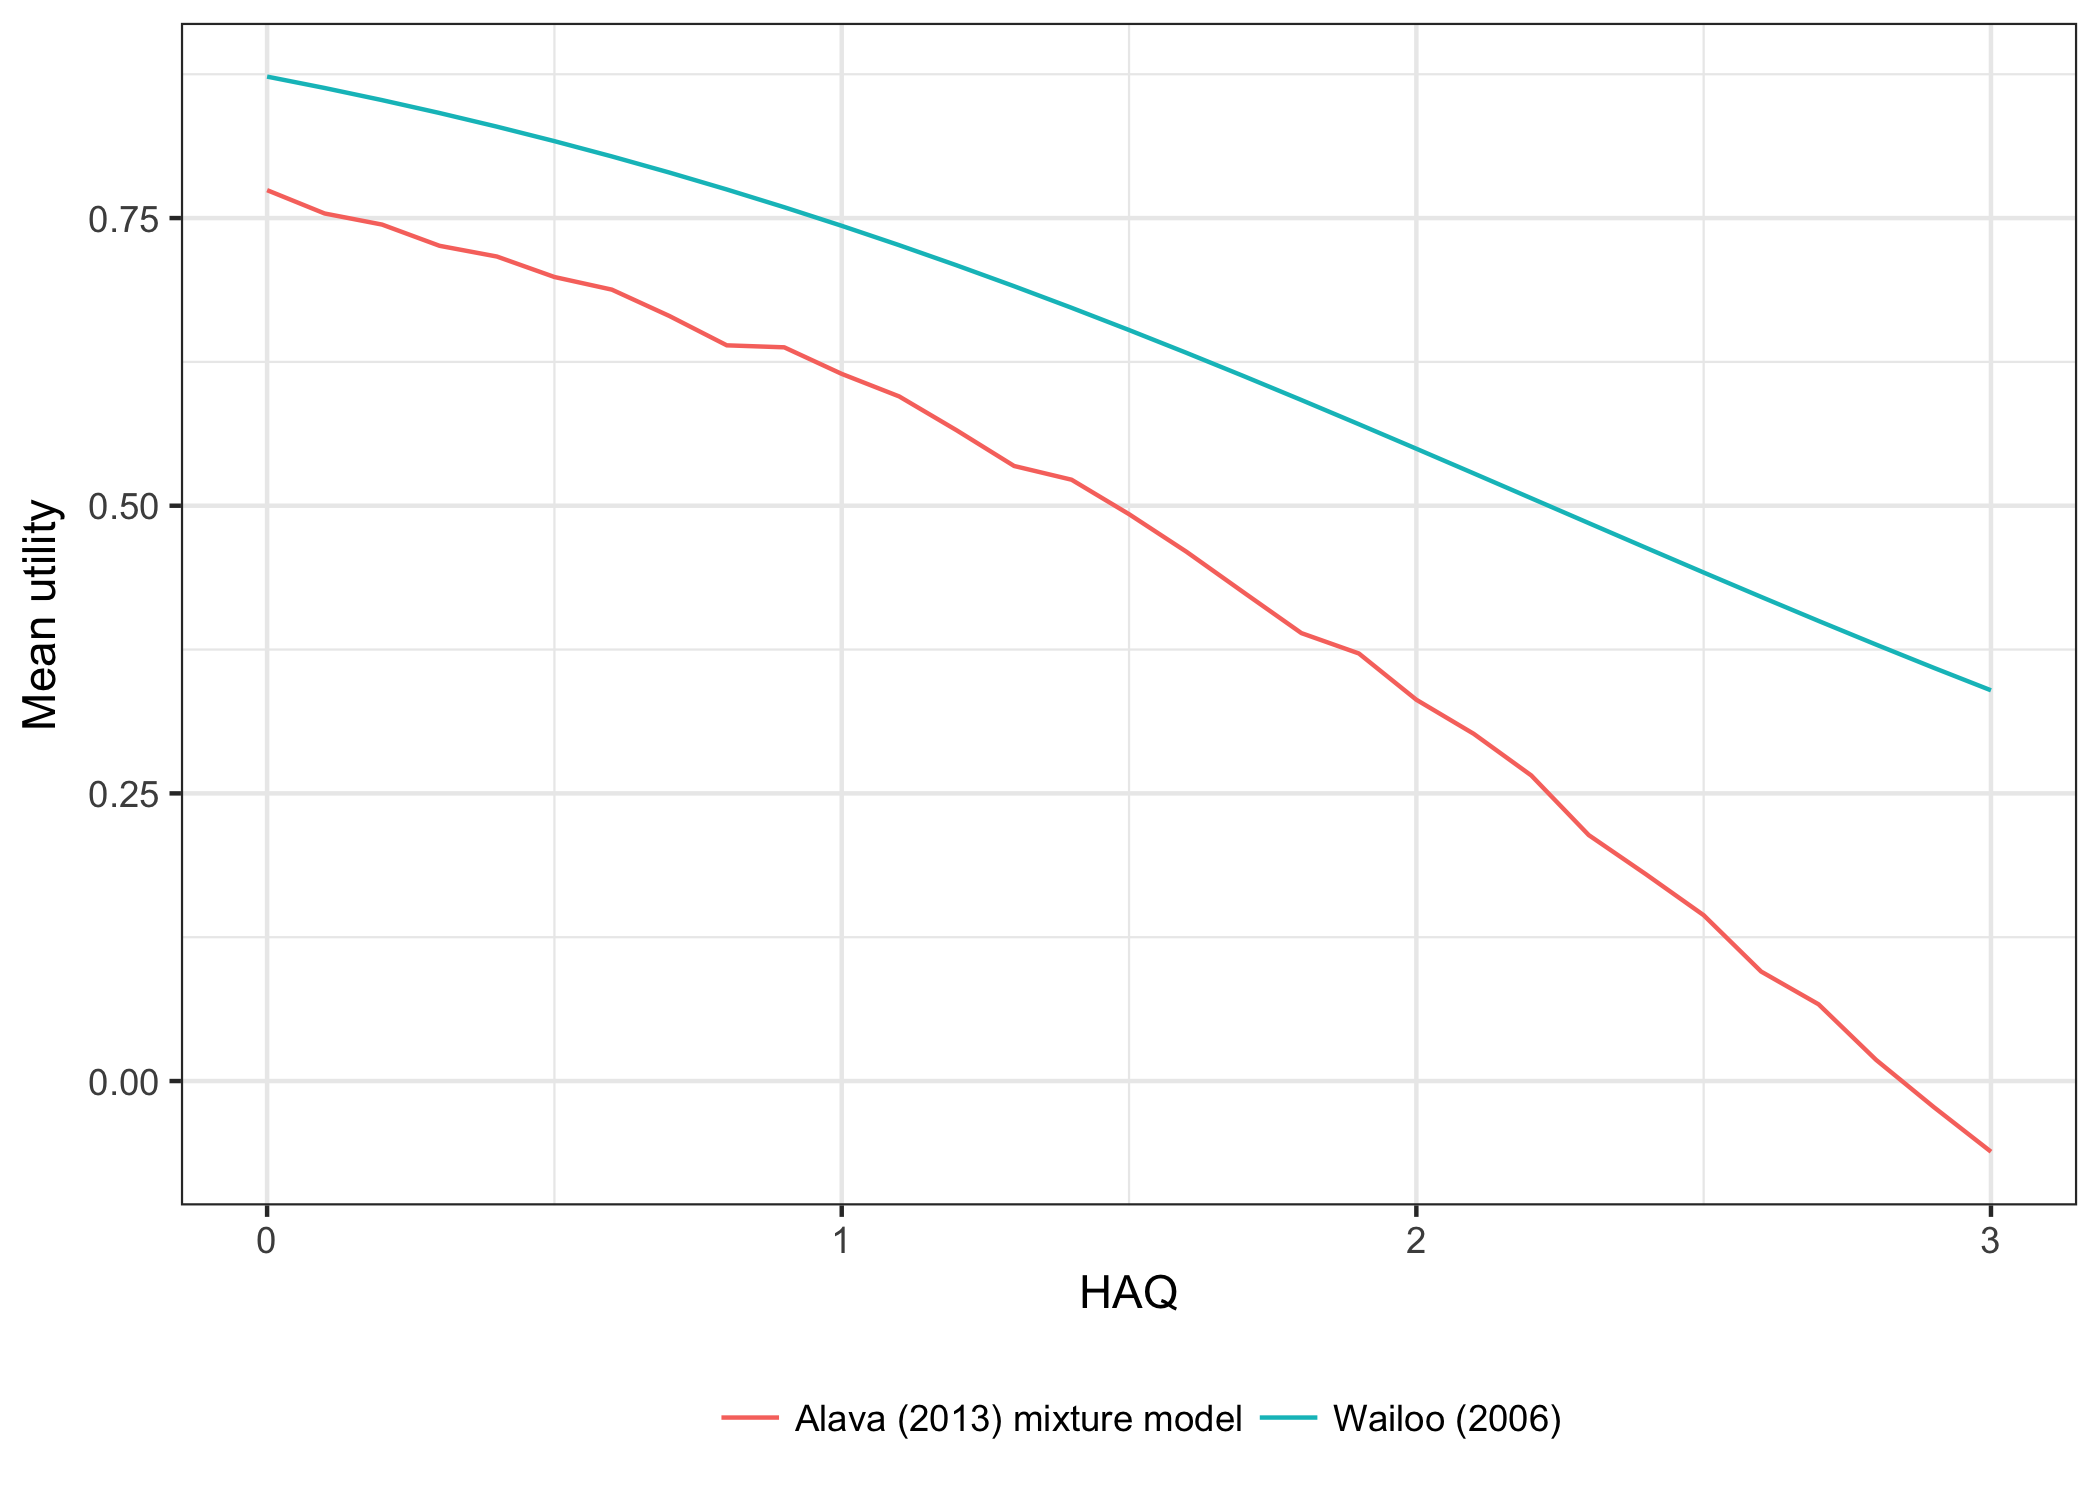
\includegraphics[max size={.8\textwidth}{.8\textheight}]{figs/util-byhaq-comparison.png}
\caption{Simulated mean utility by current
HAQ}\label{fig:util-comparison}
\end{figure}

The utility score depends on serious infections in addition to HAQ. In particular, disutility due to serious infections is assumed to be 0.156 for the duration of the month of infection based on prior studies \citep{stevenson2016adalimumab, oppong2013impact}. However, given the weak evidence for this estimate, the disutility of an infection is allowed to vary by 20\% in either direction. 

\subsection{Mortality}
The probability of death is simulated as a function of age/sex specific mortality from U.S. lifetables \citep{arias2015united}, baseline HAQ, and changes in HAQ from baseline. \citet{wolfe2003predicting} estimate an odds ratio for the effect of HAQ on mortality of 2.22, which is applied to the absolute mortality rates of the general population (HAQ score of 0). To capture the effect of treatment on mortality, we assume that, for every 0.25-unit increase in HAQ score, subsequent 6-month mortality increases according to the hazard ratios reported in \citet{michaud2012mortality}. Parameter estimates are shown in \autoref{tbl:mortpars}.



\begin{table}[!ht]
\begin{center}
\begin{threeparttable}
\caption{Mortality parameters} \label{tbl:mortpars}
\footnotesize
\begin{tabularx}{\textwidth}{@{\extracolsep{\fill}}lcccc}
\hline
\multicolumn{2}{l}{} & \multicolumn{2}{c}{95\% CI} & \multicolumn{1}{l}{} \\
\cmidrule{3-4} 
\multicolumn{1}{l}{} & \multicolumn{1}{l}{Estimate} & \multicolumn{1}{c}{Lower} & \multicolumn{1}{c}{Upper} & \multicolumn{1}{c}{Reference} \\
\hline
Impact of baseline HAQ on mortality \\
\ExpandableInput{tables/mort-or.txt}
Impact of 0.25-unit change in HAQ from baseline on mortality\\
\ExpandableInput{tables/mort-hr-haqdif.txt}
\hline
\end{tabularx}
\scriptsize
Notes: 95\% confidence intervals are calculated using normal distributions on the log odds
and log hazard ratio scales. 
\end{threeparttable}
\end{center}
\end{table}



\autoref{fig:surv} plots survival curves by gender for $1,000$ patients with a baseline age of 55. Survival was simulated by setting the log odds ratios and log hazard ratios from \autoref{tbl:mortpars} equal to their point estimates. Three scenarios are considerd. In scenario one, patients do not have RA (i.e., HAQ score of 0). In the second scenario, patients have baseline HAQ score of 1 but it does not increase over time. In the third scenario, patients still have a baseline HAQ score of 1, but it increases by 0.03 per year. The third scenario, therefore, utilizes the relationship between changes and HAQ and mortality from \citet{michaud2012mortality} while the second scenario does not. 

Mean survival for females without RA was 82.5 years and declined to 77.0 for females with a constant baseline HAQ of 1 and to 72.4 when HAQ increased by 0.03 per year. Mean survival for males in the first, second, and third scenario were 79.4, 73.2, and 70.1 years respectively. Overall, the figure suggests that RA increases mortality and that larger increases in HAQ over time increase mortality by even more.

\begin{figure}[H]
\centering
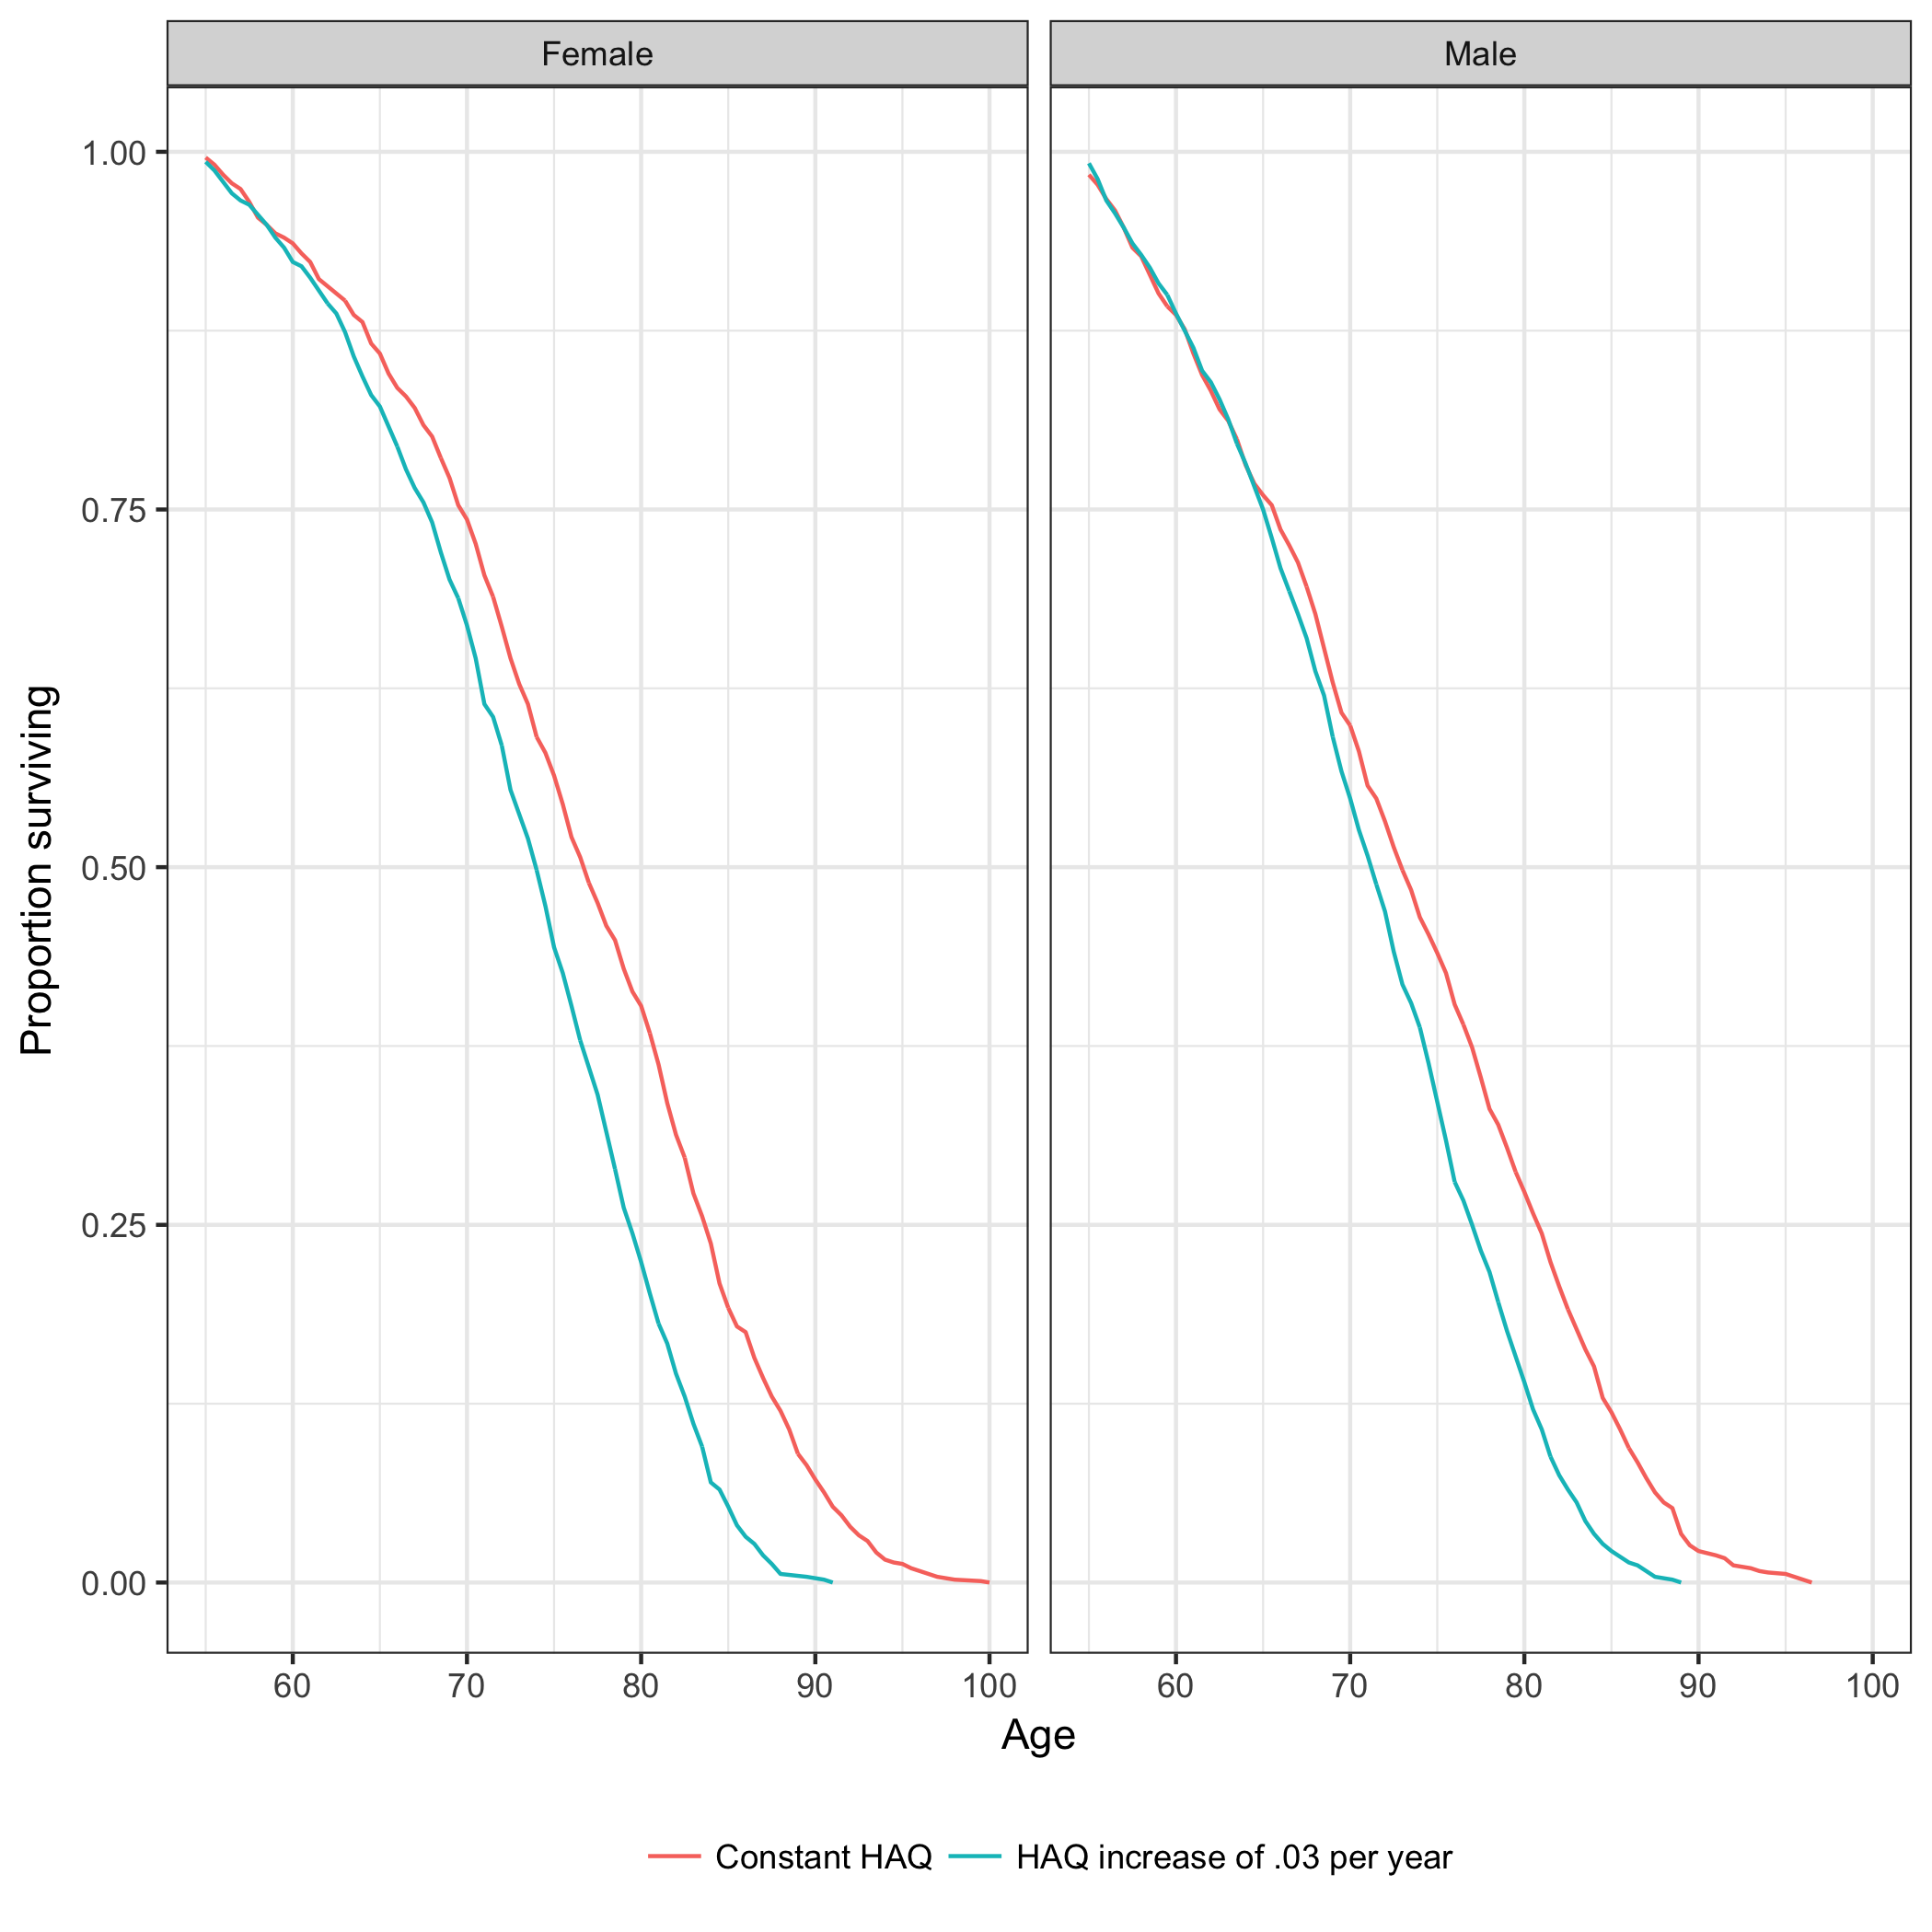
\includegraphics[max size={.7\textwidth}{.7\textheight}]{figs/surv.png}
\caption{Simulated survival curve for a patient age 55}\label{fig:surv}
\begin{minipage}{\linewidth}
\footnotesize
Notes: Baseline HAQ is 1 for the ``Constant HAQ'' and ``HAQ increase of 0.03 per year'' scenarios; baseline HAQ is 0 for the ``No RA'' scenario.
\end{minipage}
\end{figure}

\FloatBarrier

\subsection{Cost}\label{cost}


An overview of drug acquisition and administration costs is presented in \autoref{tbl:treat-cost}. Costs are a function of dose and frequency of administration, strength and dosage form, price, and infusion costs. Since infliximab dosing depend on patient weight, the costs for infliximab reported in the table average over a patient population that is 21\% male. The prices in the table are based on the wholesale acquisition cost (WAC) and do not include discounts or rebates so they may be higher than actual drug costs. In the simulation, a unique discount can be used for each drug; currently the discount is assumed to range from 20\% to 30\%. The methodology used to calculate drug acquisition and administration costs is described in more detail in \autoref{app:treat-cost}. 

\begin{sidewaystable}
\begin{center}
\begin{threeparttable}
\caption{Drug acquisition and administration cost} \label{tbl:treat-cost}
\scriptsize
\begin{tabular}{lp{0.15\linewidth}p{0.15\linewidth}rrrrrr}
\hline
\multicolumn{1}{l}{Drug} &
\multicolumn{1}{p{0.15\linewidth}}{Dose and frequency of administration} & 
\multicolumn{1}{p{0.15\linewidth}}{Strength and dosage form} & 
\multicolumn{1}{p{0.08\linewidth}}{Number of doses first 6 months}  & 
\multicolumn{1}{p{0.08\linewidth}}{Number of dosees per year beyond the first 6 months} & 
\multicolumn{1}{c}{Price per unit} & \multicolumn{1}{c}{Infusion cost} & 
\multicolumn{1}{p{0.08\linewidth}}{Cost for the first 6 months} &
\multicolumn{1}{p{0.08\linewidth}}{Cost per year beyond the first 6 months}\\
\hline
\ExpandableInput{tables/treat-cost.txt}
\hline
\end{tabular}
\tiny
Notes: Costs in the table do not include rebates or discounts, but rebates and discounts are used in the simulation. Cost for infliximab are calculated by assuming that 21\% of patients are male and that the weight of men and women are 89 kg and 75 kg respectively. Tocilizumab is dosed weekly if weight is greater than 100 kg; costs for tocilizumab reported in the table are for patients weighing less than 100 kg. IV = intravenous; SC = subcutaneous; WAC = wholesale acquisition cost. 
\end{threeparttable}
\end{center}
\end{sidewaystable}

Parameters associated with resource use are show in in \autoref{tbl:resource-use-pars}. Costs related to physician visits, chest X-rays, tuberculosis tests, and outpatient follow-up are based on \citet{claxton2016economic}. The cost per hospital day and the relationship between the HAQ score and the annual number of hospital days are from \citet{carlson2015economic}. Cost of any serious infection are assumed to be equal to the cost of pneumonia hospitalization at \$5,873, based on Medicare reimbursement rates. \citet{wolfe2005household} provide an estimate of annual income loss in relation to HAQ scores: \$4,372 (95\% CI: 2,078 to 6,607; 2002 dollars) change per unit HAQ change, which are inflated to 2016 dollars.



\begin{table}[H]
\begin{center}
\begin{threeparttable}
\caption{Resource use parameters} \label{tbl:resource-use-pars}
\footnotesize
\begin{tabularx}{\textwidth}{@{\extracolsep{\fill}}lcccc}
\hline
\multicolumn{2}{l}{} & \multicolumn{2}{c}{95\% CI} & \multicolumn{1}{l}{} \\
\cmidrule{3-4} 
\multicolumn{1}{l}{} & \multicolumn{1}{l}{Estimate} & \multicolumn{1}{c}{Lower} & \multicolumn{1}{c}{Upper} & \multicolumn{1}{c}{Reference} \\
\hline
Days in hospital per year \\
\ExpandableInput{tables/hosp-days-haq.txt}
\ExpandableInput{tables/hosp-cost-perday.txt}
General management cost \\
\ExpandableInput{tables/mgmt-cost.txt}
Productivity loss \\
\ExpandableInput{tables/prod-loss.txt}
\hline
\end{tabularx}
\scriptsize
Notes: 95\% confidence intervals for hospital days per year by HAQ score and hospital cost per day are calculated by using the methods of moments to generate the parameters of the gamma distribution given a mean and standard error. The 95\% confidence intervals for general management costs are based on normal distributions as assumed in \citet{claxton2016economic}. 95\% confidence interval for productivity loss are calculated using a normal distribution and inflated to 2016 dollars. 
\end{threeparttable}
\end{center}
\end{table}

\section{Simulation and uncertainty analysis}\label{sec:sim-uncertainty}

\subsection{Individual patient simulation}\label{individual-patient-simulation}

The IPS is a discrete-time simulation that simulates individual patients one at a time. Model cycles, denoted by $t$, were chosen to be 6-months long to be consistent with most RCT and real-world data evidence. \autoref{alg:IPS} describes the main components of the IPS for a single patient and a single treatment. The full simulation cycles through each treatment in a treatment sequence and through each simulated patient.

\begin{algorithm}
\caption{Main components of the individual patient simulation}
\label{alg:IPS}
\begin{enumerate}
\item \textbf{First 6 months ($t = 0$)}
\begin{enumerate}
\item Simulate treatment switching using \textbf{S1-S6}, time to serious infection $T_{si}$, and death (\autoref{ssec:simulating-death}).
\begin{enumerate}
\item \textbf{If} \textbf{S1-S6} leads to a treatment switch or if the sampled time to serious infection occurs during cycle 0 (i.e., $T_{si} = 0$), \textbf{then} stop treatment. It is assumed that HAQ does not change.
\newline \textbf{Else}, continue treatment. Simulate change in HAQ using \textbf{H1-H3} and time to treatment discontinuation $T$.
\item \textbf{If} patient died, \textbf{then} move to next patient. 
\end{enumerate}
\end{enumerate}
\item \textbf{Maintenance phase} (for $t > 0 \text{ and } t \leq T$)
\begin{enumerate}
\item Simulate death and change in HAQ.
\item \textbf{If} patient died, \textbf{then} move to next patient.
\item \textbf{If} $t = T$, \textbf{then} switch treatment. Treatment switch caused by a serious infection if time to serious infection occurred during or before cycle T (i.e., $T_{si} \leq T$). 
\end{enumerate}
\end{enumerate}
\end{algorithm}

\subsection{Parameter uncertainty}\label{parameter-uncertainty}
Parameter uncertainty is quantified using PSA, which propagates uncertainty in the model input parameters throughout the model by randomly sampling the input parameters from their joint probability distribution \citep{baio2015probabilistic, claxton2005probabilistic}. Probability distributions are determined according to the distributional properties of the statistical estimates, which, in turn, depend on the statistical techniques used and the distributions of the underlying data. We, for the most part, use normal distributions for sample means, gamma distributions for right-skewed data (e.g., hospital costs), and Dirichlet distributions for multinomial data. The multivariate normal distribution is used for regression parameters estimated using frequentist techniques, provided that the variance-covariance from the statistical analysis is available. For parameters estimated using a Bayesian NMA, we fit multivariate normal distributions to the posterior distribution of the parameters generated from the Markov-Chain Monte-Carlo (MCMC) algorithm using sample means and the sample covariance matrix. When we lack evidence on a parameter, we typically assume a uniform distribution with lower and upper limits that reflect the degree of uncertainty in the parameter. The PSA parameter distributions are summarized in \autoref{tbl:psa-dists}. 

\begin{table}[!ht] 
\begin{center}
\begin{threeparttable}
\caption{Probabilistic sensitivity analysis parameter distributions} \label{tbl:psa-dists}
\def\arraystretch{1.5}
\begin{tabularx}{\textwidth}{@{\extracolsep{\fill}}p{.65 \linewidth}p{.35 \linewidth}}
\hline
\multicolumn{1}{l}{Parameter(s)} & \multicolumn{1}{l}{Distribution} \\
\hline
Rebound factor & Uniform\\
NMA parameters - ACR response & Multivariate normal \\
NMA parameters - DAS28 & Multivariate normal \\
NMA parameters - HAQ & Multivariate normal \\
Drug acquisition and administration cost & Fixed \\
Survival model parameters for treatment duration during maintenance phase & Multivariate normal \\
US lifetable mortality rates & Fixed \\
Mortality probability odds ratio - baseline HAQ & Normal \\
Mortality probability hazard ratio - change in HAQ from baseline & Normal\\
ACR response to EULAR response mapping & Dirichlet \\
ACR response to SDAI mapping & Uniform \\
ACR response to CDAI mapping & Uniform \\
ACR response to HAQ mapping & Normal \\
EULAR response to HAQ mapping & Normal \\
Linear HAQ progression - by therapy & Normal \\
Linear HAQ progression - by age & Normal \\
Latent class growth model for HAQ progression & Normal \\
Utility model - \cite{alava2013relationship} mixture model & Multivariate normal \\
Utility model - \citet{wailoo2006modeling} & Normal \\
Hospital costs - hospital days by HAQ & Gamma \\
Hospital costs - hospital costs per day & Gamma \\
General management cost & Gamma \\
Serious infection - survival parameters & Normal \\
Serious infection - cost per infection & Uniform \\
Serious infection - utility loss & Uniform \\
\hline
\end{tabularx}
\scriptsize
%Notes: 
\end{threeparttable}
\end{center}
\end{table}


\subsection{Structural uncertainty}\label{stuctural-uncertainty}
We consider structural uncertainty due to two factors:

\begin{itemize}
\item The relationship between health states within the model.
\item The statistical model used to estimate parameters.
\end{itemize}

\autoref{tbl:competing-structures} summarizes the competing model structures, which are conditional on the perspective of the decision maker. In total, there are 12 x 2 x 7 x 2 = 336 possible model structures. The choice of model structure for the initial treatment phase (\textbf{H1-H3} and \textbf{S1-S6}) depends on the preferred measures of disease activity included in the model as well as whether statistical relationships should be modeled directly or indirectly. Likewise, model structures related to HAQ progression, treatment duration, and converting HAQ to utility all reflect uncertainty in the appropriate statistical model. 

\renewcommand{\arraystretch}{1.5}

\begin{table}[!ht]
\begin{center}
\begin{threeparttable}
\caption{Competing model structures} \label{tbl:competing-structures}
\begin{tabular}{p{0.80\linewidth}p{0.20\linewidth}}
\hline
\multicolumn{1}{c}{Component of model structure} & \multicolumn{1}{c}{Possible combinations} \\
\hline
Initial effect of treatment on HAQ (\textbf{H1-H3}) and switching (\textbf{S1-S6}) & 12  \\
HAQ trajectory & 2 \\
Probability distribution for treatment duration & 7 \\
Utility algorithm & 2 \\
\hline
\end{tabular}
\end{threeparttable}
\end{center}
\end{table}\renewcommand{\arraystretch}{1}


\subsection{Implementation}\label{implementation}
We begin by describing the simulation procedure conditional on model structure, which uses PSA to capture uncertainty within but not between models. The procedure proceeds in two steps: first, model parameters are sampled from their joint probability distribution (\autoref{parameter-uncertainty}), and second, for each parameter set, model outcomes are simulated one at a time for individual patients in the specified population (\autoref{sec:populations}).   

Analysts who wish to expand the analysis to capture uncertainty between models can follow the approach described in \citet{bojke2009characterizing}. In particular, for each randomly sampled parameter set, each model structure (or a subset of plausible model structures) can be simulated. The distribution of simulated outcomes across parameters and models will then reflect uncertainty both within and between models. 

It's important to note that simulation output for an individual patient captures differences in outcomes across patients due to random variation (often referred to as first order uncertainty). This information might be useful to patients since it is needed to predict the distribution of their future outcomes conditional on their characteristics, but less useful to a decision maker concerned with making treatment decisions for a population or subset of a population. Analysts wishing to use the model for CEA should therefore estimate mean outcomes by averaging over the simulated patients for each parameter set and model structure. The number of simulated patients should be sufficiently large so that mean outcomes are stable across model runs (i.e., so that first order uncertainty is eliminated). 

Although CEA is concerned with mean outcomes, that does not imply that it does not account for heterogeneity. Instead, since outcomes depend on the characteristics of each patient, model averages are a function of the population analyzed. Subgroup analyses can be used to examine differences in cost-effectiveness across subgroups by simulating patients with certain shared characteristics. 

Parameter and structural uncertainty imply decision uncertainty, or the degree to which decisions are made based on imperfect knowledge. Indeed, with the aim to maximize health outcomes for a given budget, the optimal decision with current information is to choose the policy that maximizes the expected NMB; however, due to uncertainty, the incorrect policy may be considered the most cost-effective. To characterize this uncertainty, standard summary measures including 95\% credible intervals for NMBs and other model outcomes, cost-effectiveness planes, and cost-effectiveness acceptability curves, and the expected value of perfect information can be calculated from the simulated output. Since the expected value of partial perfect information is computationally costly, it can be approximated using meta-modeling techniques \citep{jalal2013linear, jalal2015computing, heath2016estimating}.

\section{Validation}\label{sec:validation}
We aim to validate the model using the five types of validation described by \citet{eddy2012model}. Currently, we are able to use the first three validation types. First, we have checked the model for face validity by ensuring that simulated outcomes are consistent with current science and evidence. Second, we performed unit tests to verify that the individual units of code that are used to simulate the model return expected results. Third, we compared simulated results for key outcomes such as mortality, HAQ over time, and time to treatment discontinuation with real-world data and our underlying parameter values. In particular, we ran the model online under various scenarios using our R Shiny web application and checked the simulated outcomes. 

In the future, we plan to use both external validation and predictive validation to help fine tune our model. External validation will be performed by comparing outcomes simulated using our model to real-world outcomes and predictive validity will involve using our model to forecast future events and comparing our forecasted outcomes to the observed outcomes. 

\section{Limitations and areas for improvement}\label{sec:limitations}
The IVI-RA model is an open-source model that is meant to be updated and improved over time. We believe that there are number of potential areas for improvement.

\begin{itemize}
\item \textbf{Adverse events other than serious infections:} The current model does not account for side effects other than serious infections even though these are important to patients and can result in treatment switching. 
\item \textbf{Adverse events that vary across biologics:} The model allows the serious infection rate to differ between cDMARDs and bDMARDs but assumes that the infection rate is equal among bDMARDs. Future model versions might want to reconsider the evidence underlying this assumption.
\item \textbf{Time to treatment discontinuation:} Our time to treatment discontinuation curves are based on scanned data and combine information from multiple sources. Direct analyses of databases like the CORRONA database or the National Data Bank for Rheumatic Diseases (NDB) could generate more accurate estimates of treatment duration as well the effect of treatment response or disease activity level on discontinuation rates.  
\item \textbf{Patient preferences:} In the current model, patient utility is a function of the HAQ score and varies according to age, gender, and unobserved patient-specific factors. In other words, utility depends on treatment (through the effect of treatment on HAQ) and the characteristics of the patient. Future iterations of the model should consider other ways that treatment influences utility and that utility varies across patients. For example, disease activity level or the number of previous therapies might help predict utility conditional on HAQ. Furthermore, surveys could be used to estimate the effect of treatment attributes such as route of administration or frequency of administration on utility. Finally, since unobserved patient-specific factors are very important predictors of utility, the model could be run for specific classes of patients within the mixture model (e.g., subgroups where HAQ has the largest effect on utility), although it might be difficult to identify these patient subgroups in a real-world setting. 

\item \textbf{Treatment effect modifiers:} There is currently little evidence (that we are aware of) suggesting that treatment effects vary across patients. When there is sufficient evidence in the literature related to treatment response heterogeneity, we will allow treatment response at 6 months to depend on the characteristics of the patient.  
\item \textbf{Treatment effects after treatment failure:} There are two main limitations in the model related to reductions in treatment response after failing a biologic; first, there are not enough RCTs to reliably estimate bDMARD-specific treatment effects for bDMARD experienced patients using a NMA, and second, treatment response likely does not only depend on whether a patient is bDMARD naive or experienced, but on the number of previous failures as well. Our current approach is to assume that treatment response is reduced for bDMARD experience patients based on evidence from \citet{carlson2015economic}. One possible extension is to use a Bayesian NMA approach in which the \citet{carlson2015economic} results are used to generate priors for the bDMARD experienced group. As new RCTs become available, the posterior distributions from the Bayesian analysis would move further from the prior and closer to estimates from the trials. The estimates could be further improved by combing NMA results with real-world data and modeling reductions in treatment response as a flexible function of the number of failed biologics. 
\item \textbf{A LCGM for the progression of bDMARDs over time:} The LCGM can be used to model HAQ progression for patients using cDMARDs or on NBT; however, we only have estimates of constant linear progression of HAQ for patients on bDMARDs. Future studies that use non-linear mixture models to model the long-term progression of disease for patients using bDMARDs are needed. 
\item \textbf{The patient population:} Our population characteristics are based on summary data reported in the published literature. As a result, the sampled patient populations within the model do not account for correlations across all of the variables. Distributions estimated from patient databases like the CORRONA database or the NDB would yield more realistic patient populations. 
\item \textbf{Estimating the rebound effect:} One of the most important predictors of cost-effectiveness is the degree to which the HAQ score increases following treatment failure. Most models currently assume that the HAQ score increases by the same amount as the initial 6 month decline in the HAQ score, but there is little evidence to support this. Studies that attempt to quantify the rebound effect are critical. 
\end{itemize}

\begin{appendices}
\setcounter{table}{0}
\renewcommand{\thetable}{A\arabic{table}}
\setcounter{figure}{0}
\renewcommand{\thefigure}{A\arabic{figure}}
\setcounter{equation}{0}
\renewcommand{\theequation}{A\arabic{equation}}

\section{Rates, probabilities, and standard errors}\label{app:math}
\subsection{Using odds ratios to adjust probabilities}\label{app:odds-ratio-prob}
Let $p_1$ be a baseline probability, $\beta$ be a vector of log odds ratios, and $x$ be a vector of regressors. We apply the log odds ratios to $p_1$ to generate a new probability $p_2$ with the logistic equation,

\begin{align}
p_2 &= \frac{1}{1 + \exp\left[-\left(\logit(p_1) + x^T\beta \right)\right]},
\end{align}

where,

\begin{align}
\logit(p) = \log\left(\frac{p}{1-p}\right)
\end{align}

\subsection{Converting rates and probabilities}\label{app:rate-prob}
Given a \emph{constant} rate $r$ during a given time period, we estimate the probability of an event occurring before time $t$ using the exponential distribution,

\begin{align}
p(\tau < t |r) &= 1 - e^{-rt}.
\end{align}

Given a probability $p$, the rate parameter is recovered by applying the log transformation,

\begin{align}
r = \frac{-\ln(1-p)}{t}.
\end{align}

\subsection{Calculating standard errors from confidence intervals}\label{app:ci-se}
Journal articles often report confidence intervals rather than standard errors. However, given that regression coefficients are asymptotically normally distributed, standard errors can be calculated from a confidence interval using the normal distribution. In particular, given a coefficient estimate $\beta$ (e.g., a log hazard ratio, log odds ratio, or linear regression coefficient) and an upper bound $u$ and lower bound $l$ of a two-sided 95\% confidence interval, we calculate the standard error as,

\begin{align}
SE(\beta) = \frac{u - l}{2 \cdot \Phi^{-1}(0.975)},
\end{align}

where $\Phi^{-1}(p)$ is the quantile function of the normal distribution. 


\section{Heterogeneous populations}\label{app:population}
When generating heterogeneous patient populations, we sample binary variables from binomial distributions, continuous uncorrelated variables from normal distributions, and continuous correlated variables from multivariate normal distributions. Truncated distributions are used when variables are restricted to lie within certain intervals. 

In particular, the proportion of the female population is drawn from a binomial distribution while age, disease duration and the number of previous DMARDs are drawn from truncated normal distributions. Each sampled value of the number of previous DMARDs is rounded to the nearest integer. Baseline HAQ and three disease activity measures (DAS28, SDAI, and CDAI) are drawn from truncated multivariate normal distributions. The covariance matrix is calculated using the correlations reported in \citet{aletaha2005acute} (\autoref{fig:da-cor}).



\begin{figure}[H]
\centering
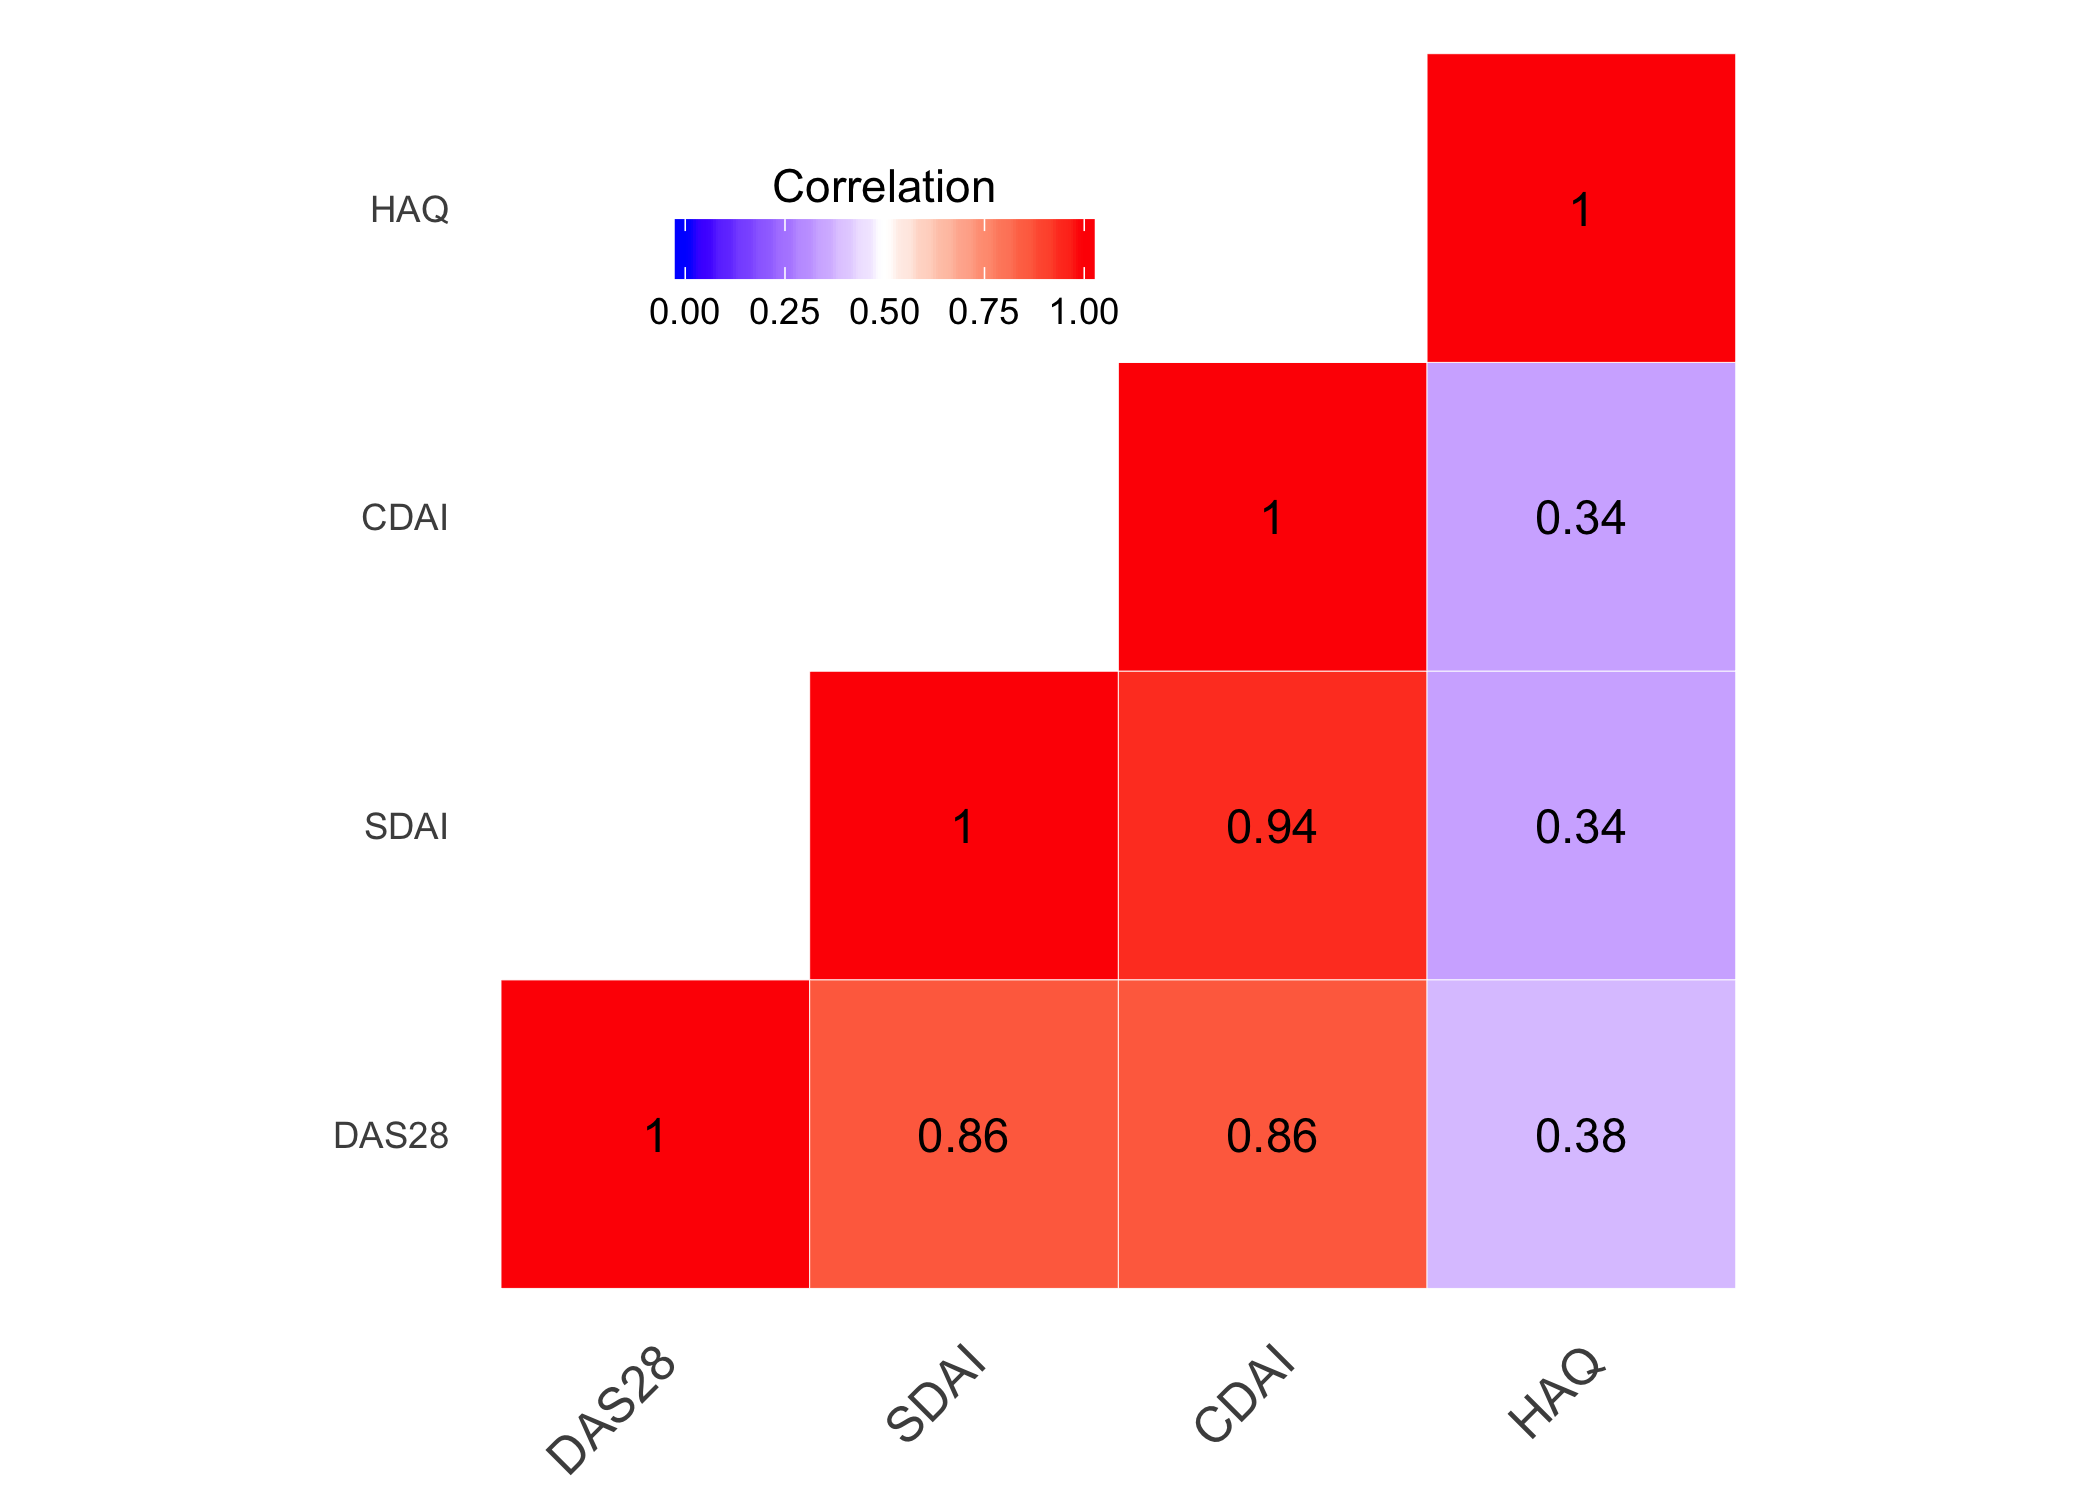
\includegraphics[max size={.7\textwidth}{.7\textheight}]{figs/da-cor.png}
\caption{Correlations between disease activity measures and HAQ}\label{fig:da-cor}
\end{figure}

We used the correlations from the routine cohort (during visit 1) rather than correlations in the inception cohort (at baseline) since the correlation between HAQ and the disease activity measures were more similar to those from the Leflunomide database \citep{smolen2003simplified}. That said, correlations between the three disease activity measures were nearly identical in each cohort. The one exception was that the correlation between SDAI and CDAI of 1 in the routine cohort seemed unreasonably high so we used the value of 0.94 from the inception cohort. 




We used this sampling procedure to simulate 1,000 patients. Summary statistics from a simulated patient cohort of size 1,000 are shown in \autoref{tbl:pats-samp}.

\begin{table}[!ht]
\begin{center}
\begin{threeparttable}
\caption{Summary of characteristics for 1,000 simulated patients} \label{tbl:pats-samp}
\begin{tabularx}{\textwidth}{@{\extracolsep{\fill}}lccc}
\hline
\multicolumn{2}{c}{} & \multicolumn{2}{c}{95 CI\%} \\
\cmidrule{3-4}
\multicolumn{1}{l}{} & \multicolumn{1}{c}{Mean} & \multicolumn{1}{c}{Lower} & \multicolumn{1}{c}{Upper}\\
\hline
\ExpandableInput{tables/pats-samp.txt}
\hline
\end{tabularx}
\scriptsize
\end{threeparttable}
\end{center}
\end{table}

\section{Mapping ACR response to changes in disease activity}\label{app-acr-da}
Let $DA$ denote disease activity, $n_1$ the number of patients with ACR 20 to <50 response, $n_2$ the number of patients with ACR 50 to <70 response, $n_3$ the number of patients with ACR $\geq$70 response, and $N$ the number of patients with an ACR response greater than or equal to 20\%. Mean changes in SDAI, CDAI, and DAS28 by overlapping ACR response categories are converted to mean changes by mutually exclusive ACR response categories as follows:

\begin{itemize}
\item \textbf{ACR 70}: Mean changes by ACR $\geq$70 were reported directly in \citet{aletaha2005simplified}.
\item \textbf{ACR 50 to <70}: Mean change in disease activity given ACR 50 to <70 response is calculated by solving for $\E[DA|50 \leq ACR < 70]$:

\begin{align}
\E[DA|ACR \geq 50] = \frac{n_2}{N} \cdot \E[DA|50 \leq ACR < 70]  + \frac{n_3}{N} \cdot \E[DA|ACR \geq 70].
\end{align}

\item Mean change in disease activity given ACR 20 to <50 response is calculated by solving for $\E[DA|20 \leq ACR < 50]$

\begin{align}
\E[DA|ACR \geq 20] = \frac{n_1}{N} \cdot \E[DA|20 \leq ACR < 50]  + \frac{n_2 + n_3}{N} \cdot \E[DA|ACR \geq 50].
\end{align}

\end{itemize}

\section{HAQ progression}\label{app:haq-progression}
\subsection{Effect of age on linear HAQ progression}\label{app:age-linear-haq}
\citet{michaud2011treatment} report an overall rate of linear HAQ progression and rates for three age groups (<40, 40-64, $\geq$ 65). Let $\beta$ be the overall rate of progression and $\beta_a$ be the rate of progression for age group $a$. To estimate the effect of age on the progression rate, we calculated the difference between the overall progression rate and the age specific rate, $\delta_a = \beta - \beta_a$. We estimated the standard error of this quantity assuming no covariance between $\beta$ and $\beta_a$,

\begin{align}
SE(\delta_a) = \sqrt{SE(\beta)^2 + SE(\beta_a)^2}.
\end{align}


\subsection{HAQ trajectory with a latent class growth model}\label{app:lcgm-haq}
\citet{norton2014health} model HAQ progression using a LCGM. The probability that individual $i$ is a member of class $c$ at time $t$ is modeled using a multinomial logistic regression,

\begin{align}
P(C_{it} = c) &= \frac{\exp(w_{it}^T\delta_c)}{\sum_{s=1}^{4}\exp(w_{it}^T\delta_s)},
\end{align}

where $\delta_s$ is the vector of regression coefficients associated with class $s$ and $w_{it}$ is the corresponding vector of regressors. The variables included in $w_{it}$ are age, gender, baseline DAS28, symptom duration, rheumatoid factor, ACR criteria, and socioeconomic status. Regression coefficients for classes 2-4 relative to class 1 are shown in \autoref{tbl:lcmm-class-coefs}. Older age and female gender are especially important predictors of membership in higher risk classes; a worse DAS28 score, rheumatoid factor positivity, fulfillment of the 1987 ACR criteria, lower socioeconomic status, and longer disease duration are also predictors of membership in classes with worse HAQ progression. 



\begin{table}[!ht] 
\begin{center}
\begin{threeparttable}
\caption{Determinants of class membership in the ERAS cohort} \label{tbl:lcmm-class-coefs}
\begin{tabularx}{\textwidth}{@{\extracolsep{\fill}}lccc}
\hline
\multicolumn{2}{l}{} & \multicolumn{2}{c}{95\% CI} \\
\cmidrule{3-4} 
\multicolumn{1}{l}{} & \multicolumn{1}{c}{Coefficient} & \multicolumn{1}{c}{Lower} & \multicolumn{1}{c}{Upper}  \\
\hline
\multicolumn{4}{@{}l}{\textbf{Class 2: moderate}} \\
\ExpandableInput{tables/lcgm-coef-class2.txt} \\
\multicolumn{4}{@{}l}{\textbf{Class 3: high}} \\
\ExpandableInput{tables/lcgm-coef-class3.txt} \\
\multicolumn{4}{@{}l}{\textbf{Class 4: severe}} \\
\ExpandableInput{tables/lcgm-coef-class4.txt}
\hline
\end{tabularx}
\scriptsize
Notes: Class 1, or the "low" group, is the reference category.
\end{threeparttable}
\end{center}
\end{table}

The HAQ trajectory for a given class can be written as,

\begin{align}\label{eqn:lcgm-haq}
y_{itc}^{*} &= \beta_{0c} + \beta_{1c}x_t + \beta_{2c}x_t^2 + \beta_{3c}x_t^3 + \epsilon_{it} \\
y_{itc} &= 
\begin{cases}
  0 & \text{if}\  y_{itc}^{*} < 0 \\
  y_{itc}^{*}& \text{if}\  0 \leq y_{itc}^{*} \leq 3 \\
   3 & \text{if}\  y_{itc}^{*} > 3 ,
\end{cases}
\end{align}

where $y_{itc}$ is the HAQ score, $x_t$ is a variable that is a function of time, the $\beta_{jc}$ are polynomial regression coefficients for members of class c, and $\epsilon_{it}$ is an error term.

Sam Norton generously provided us with statistical estimates of the 4 class LCGM used in \citet{norton2014health} from \href{https://www.statmodel.com}{MPlus}. Like \citet{stevenson2016adalimumab}, we noted that the coefficient estimates the MPlus resulted in large fluctuations in the predicted HAQ scores, likely because three decimal places was not precise enough for the cubic term in \autoref{eqn:lcgm-haq}. We consequently used the coefficient estimates to predict the probability of class membership---which are less likely to be influenced by the number of reported decimal places---but estimated \autoref{eqn:lcgm-haq} using the observed HAQ values reported in Figure 2 in \citet{norton2014health}. However, since standard errors were artificially high using grouped data, we standard errors in \autoref{eqn:lcgm-haq} were based on those reported in the original paper. Moreover, since we are only interested in the HAQ trajectory following the HAQ decline during the initial treatment phase, we limited our analysis to HAQ values from year 2 and onwards. Using the post year 2 data, we estimated \autoref{eqn:lcgm-haq} using separate linear regressions with cubic polynomials for each class (\autoref{tbl:lcmm-growth-coefs}). Like \citet{norton2014health}, we set $x_t$ equal to a reciprocal transformation of time,

\begin{align}
x_t &= 1 - \frac{1}{t+1}
\end{align}

\begin{table}[!ht] 
\begin{center}
\begin{threeparttable}
\caption{LCGM HAQ trajectory coefficients} \label{tbl:lcmm-growth-coefs}
\begin{tabularx}{\textwidth}{@{\extracolsep{\fill}}lccc}
\hline
\multicolumn{1}{l}{} & \multicolumn{1}{c}{Coefficient} & \multicolumn{1}{c}{Standard error}  \\
\hline
\multicolumn{3}{@{}l}{\textbf{Class 1: low}} \\
\ExpandableInput{tables/lcgm-coef-growth-class1.txt} \\
\multicolumn{3}{@{}l}{\textbf{Class 2: moderate}} \\
\ExpandableInput{tables/lcgm-coef-growth-class2.txt} \\
\multicolumn{3}{@{}l}{\textbf{Class 3: high}} \\
\ExpandableInput{tables/lcgm-coef-growth-class3.txt} \\
\multicolumn{3}{@{}l}{\textbf{Class 4: severe}} \\
\ExpandableInput{tables/lcgm-coef-growth-class4.txt}
\hline
\end{tabularx}
\scriptsize
Notes: Class 1, or the ``low'' group, is the reference category.
\end{threeparttable}
\end{center}
\end{table}

In the cost-effectiveness model, we simulate the HAQ score at 6 months as a function of the baseline HAQ score and the change in HAQ during the initial treatment phase. Since the \citet{norton2014health} model is not conditional on the HAQ score in the previous period, we use it to predict changes in HAQ rather than the level of the HAQ score. More precisely, for a patient in a given class, we model the change in HAQ as,  

\begin{align}\label{eqn:lcgm-dhaq}
\Delta y_{itc}^{*} &= y_{i,t,c}^{*} - y_{i,t-1,c}^{*} \\
&= \beta_{1c}(x_t - x_{t-1}) + \beta_{2c}(x_t^2 - x_{t-1}^2) + \beta_{3c}(x_t^3-x_{t-1}^3) + (\epsilon_{i,t} - \epsilon_{i,t-1}). \nonumber
\end{align}

Since \autoref{eqn:lcgm-haq} was estimated on aggregated data, we did not have reliable estimates of $\epsilon_{it}$. We consequently set $\epsilon_{i,t} - \epsilon_{i,t-1}$ equal to 0, which implies that we are generating a mean response rather than a predicted response. In other words, we are not simulating the random variation associated with each individual, but are still accurately simulating mean outcomes across populations or subpopulations. 

\section{Simulating death}\label{ssec:simulating-death}
Death is simulated for each patient during each model cycle based on age, gender, baseline HAQ, and change in HAQ from baseline. A 0/1 death indicator is randomly drawn using the following procedure: 
\begin{enumerate}
\item Find $q_{xg}$, the probability that a patient of gender $g$ and age $x$ will die before age $x+1$, from lifetables.
\item As described in \autoref{app:odds-ratio-prob}, adjust $q_{gx}$ using the effect of a change in baseline HAQ on the odds of mortality, $OR$,
\begin{align}
p_m = \frac{1}{1 + \exp{\left[-(\text{logit}(q_x) + \log(OR)\cdot HAQ)\right]}}.
\end{align}
\item Following \autoref{app:rate-prob}, convert the mortality probability, $p_m$, into a mortality rate, $r_m$.
\begin{align}
r_m &= -log(1 - p_m).
\end{align}
\item Adjust the mortality rate, $r_m$, using the estimated log hazard ratio of mortality, $HR$, of a change in HAQ from baseline, $\Delta$ HAQ.
\begin{align}
r_m &= r_m \cdot \exp[\log(HR) \cdot \Delta HAQ]
\end{align}
\item Following \autoref{app:rate-prob}, convert the mortality rate into a probability given a 6-month cycle length,
\begin{align}
p_m = 1 - \exp[-r_m * (6/12)].
\end{align}
\item Randomly draw a 0/1 death indicator, $d$, given the probability of death, $p_m$,
\begin{align}
d \sim \text{Bin}(1, p_m).
\end{align}
\end{enumerate}

\section{Simulating utility with a mixture model}\label{app:sim-utility-mixture}
The mixture model estimated by \citet{alava2013relationship} simulates utility in two stages. In the first stage, we sampled pain for a given individual in a particular model cycle based on the HAQ score. In the second stage, we simulated utility as a function of HAQ, pain and age/sex.

\subsection{Simulating pain}
To simulate pain from HAQ, we used the summary statistics for pain and HAQ reported in \citet{sarzi2002correlation}. Pain was measured with the visual analog scale (VAS) with mean  $\mu_{pain} =$ 61.65 and standard deviation $\sigma_{pain} =$ 19.10, while HAQ was reported to have mean $\mu_{haq} =$ 1.39 and standard deviation $\sigma_{haq} =$ 0.59. 

We then estimated the correlation between pain and HAQ by digitally scanning the curve depicting the (linear) relationship between pain and HAQ (Figure 114) shown in \citet{stevenson2016adalimumab}. Using the scanned data, we regressed pain on HAQ using simple ordinary least squares (OLS). The correlation between pain and HAQ, estimated as $\rho =$ 0.52, was calculated by rearranging the OLS estimate for the slope, $\beta$, of the regression model,

\begin{align}
\rho = \beta \cdot \frac{\sigma_{haq}}{\sigma_{pain}}.
\end{align}

Pain was simulated using these parameters by assuming that pain was normally distributed conditional on HAQ,

\begin{align}
pain | haq = h \sim N\left (\mu_{pain} + \rho \frac{\sigma_{pain}}{\sigma_{haq}}(h - \mu_{haq}), \sigma^2_{pain}(1 - \rho^2)\right).
\end{align}

However, since the VAS is constrained to lie between 0 and 100, pain was drawn from a truncated normal distribution with a lower limit of 0 and an upper limit of 100. 


\subsection{Simulating utility}
After simulating pain, we simulated utility with a mixture model. Within each class $c$, the HAQ score for patient $i$ in period $t$ was modeled as,

\begin{align}
y_{it|C_{it}} &= 
\begin{cases}
  1 & \text{if}\  y^{*}_{it|C_{it}}>0.883 \\
  y^{*}_{it|C_{it}} & \text{otherwise}
\end{cases}\\
y^{*}_{it|C_{it}} &= \alpha_{ic} +  x_{it}^T\beta_{c} + \epsilon_{it}\\
\alpha_{ic} &=  \gamma_{c} + z_{i}^T\kappa + \mu_{i},
\end{align}

where $\epsilon_{it}$ is a random error term and $\beta_{c}$ is a vector of regression coefficients corresponding to the vector of variables $x_{it}$. $\alpha_{ic}$ is a random intercept for individual $i$ and class $c$ that is predicted by a class-specific intercept, $\gamma_c$, a vector of individual-specific variables $z_{i}$, a coefficient vector $\kappa$, and an error term, $\mu_i$. Variables included in $x_{it}$ are $HAQ$, $HAQ^2$, $Pain/100$, $Age/10$, and $Age/100$; $z_{i}$ contains a single indicator variable, $Male$, equal to 1 if the patient is male and 0 if female.

The probability of class membership was modeled using a multinomial logit model,

\begin{align}
P(C_{it} = c) &= \frac{\exp(w_{it}^T\delta_c)}{\sum_{s=1}^{4}\exp(w_{it}^T\delta_s)},
\end{align}

where there are four possible classes and $\delta_c$ is a vector of coefficients corresponding to the vector of variables, $w_{it}$ (which includes an intercept). Variables included in $w_{it}$ other than the intercept are $HAQ$, $Pain/100$, and $Pain/100^2$.

We sampled from the mixture model as follows.

\begin{enumerate}
\item For each individual $i$, sample the error term, $\mu_{i} \sim N(0, \sigma^2_\mu)$.
\item For each individual $i$ and time-period $t$: 
\begin{enumerate}
\item Sample class membership conditional on $w_{it}$; that is, sample $C_{it} \sim \rm{Cat}(p_1, p_2, p_3, p_4)$ where $p_c$ is the probability of being in class $c$.
\item Predict the intercept $\alpha_{ic}$.
\item Sample the error term, $\epsilon_{it} \sim N(0, \sigma^2_\epsilon)$.
\item Predict the HAQ score, $y_{it}$. 
\end{enumerate}
\end{enumerate}

\section{Drug acquisition and administration costs}\label{app:treat-cost}


Drug acquisition and administration costs are calculated separately during the initial treatment phase and the maintenance phase since dosing typically differs. Costs are separated into acquisition costs and infusion costs. Infusion costs are calculated by multiplying the number of doses in a 6 month period by the cost of an infusion and acquisition costs are calculated as,

\begin{align}
cost = \left\lceil\frac{dose_{amt}}{strength_{amt}}\right\rceil \cdot doses_{num} \cdot WAC,
\end{align}

where $\lceil\cdot\rceil$ is the ceiling function and implies that products cannot be reused after opening, $dose_{amt}$ is the recommended dose of the drug, $strength_{amt}$ is the strength of the drug, $doses_{num}$ is the number of doses in a 6 month period, and $WAC$ is the WAC. For example, as shown in \autoref{tbl:treat-cost}, both the strength and the dose of adalimumab are 50 mg, so costs for the initial 6 month period are calculated by multiplying the number of doses (13) by the WAC (\$).

When dosing depends on weight, costs are calculated separately for each patient in the simulation. In particular, costs are calculated as,

\begin{align}
cost &= \lceil weight \cdot dose_{amt}/strength_{amt}\rceil \cdot doses_{num} \cdot WAC,
\end{align}

where $\rm{weight}$ is patient weight, $dose_{amt}$ is the dose per weight, and $strength_{amt}$, $WAC$, and $doses_{num}$ are defined in the same way as in the non-weight based scenario. To illustrate, the acquisition cost for infliximab after the first 6 months is calculated by multiplying each patient's weight by the dose (6 mg/kg) and dividing by the size of a vial (100 mg), and then multiplying by the number of doses (8.67) and the WAC (\$).  

\section{Network Meta-Analysis}\label{appendix:NMA}

\subsection{Systematic literature review}\label{systematic-literature-review}

\textbf{Population}
\begin{itemize}
\item Adult (\textgreater{}18 years) patients with moderate to severe RA who have had inadequate response to cDMARDs
\end{itemize}

\textbf{Interventions and comparators}

\begin{itemize}
\item Biologics as monotherapy or in combination with cDMARDs (adalimumab, certolizumab pegol, etanercept, golimumab, infliximab, abatacept, rituximab, tocilizumab, sarilumab, tofacitinib)

\item cDMARDs alone or in combination (MTX, HCQ, SSZ or LEF)
\end{itemize}

\textbf{Outcomes}
\begin{itemize}
\item ACR20/ACR50/ACR70
\item DAS28
\item HAQ-DI score
\end{itemize}

\textbf{Study design}
\begin{itemize}
\item Randomized controlled trials
\end{itemize}

\textbf{Other}

\begin{itemize}
\item Studies published in English
\item Primary study available as full text published manuscript only; no study available as a conference abstract only was included.
\end{itemize}

\subsection{Criteria for studies to be selected from the systematic literature review and included in the NMA}\label{criteria-for-studies-to-be-selected-from-the-systematic-literature-review-and-included-in-the-nma}

The following criteria were used to select relevant studies to be included in the NMA:

\textbf{Population}

\begin{itemize}
\item Adult (\textgreater{}18 years) patients with moderate to severe RA who have had inadequate response to cDMARDs and are bDMARD-naive
\end{itemize}

\textbf{Interventions}

\begin{itemize}
\item Biologics as monotherapy or in combination with cDMARDs (adalimumab, certolizumab pegol, etanercept, golimumab, infliximab, abatacept, rituximab, tocilizumab, sarilumab, tofacitinib)
\end{itemize}

\textbf{Comparators}

\begin{itemize}
\item cDMARDs
\item Any active comparator that allows for an indirect comparison between the bDMARDs of interest
\end{itemize}

\textbf{Outcomes}

\begin{itemize}
\item ACR20/ACR50/ACR70 at 6 months follow-up
\item Change in DAS28 from baseline at 6 months follow-up
\item Change in HAQ-DI score from baseline at 6 months follow-up 
\end{itemize}

\subsection{Identified evidence base}\label{identified-evidence-base}
%The evidence network is presented in \autoref{fig:nma-network-acr-naive}. 
The evidence network and inclusion criteria to go here.

% \autoref{fig:study-selection} summarizes the study identification and selection process. Of the 181 studies included in the large systematic literature review, 79 studies concerned the bDMARD-naive population (table NMA studies). There were 66 studies evaluating 36 interventions for which ACR response criteria were reported at 6 months (with a tolerability window of \(\pm 4\) weeks).  

% For the network meta-analysis the following were deemed to be clinically equivalent and were pooled.

% \begin{itemize}
% \item ``INF 3mg/kg q8w'' or ``INF 5mg/kg q8w'' or ``INF 6mg/kg q8w''
% \item ``ETN 50mg qw'' or ``ETN 25mg biw''
% \item ``ABA 10mg/kg q4wa or''ABA SC 125mg qw"
% \item ``CER 200mg q2w+MTX'' or ``CER 400mg q4w+MTX
% \item DMARDs including methotrexate, sulfasalazine, hydroxychloroquine, leflunomide at any dosage; studies which only described DMARD therapy as conventional or nonbiologic
% \end{itemize}

% \begin{figure}
% \centering
% 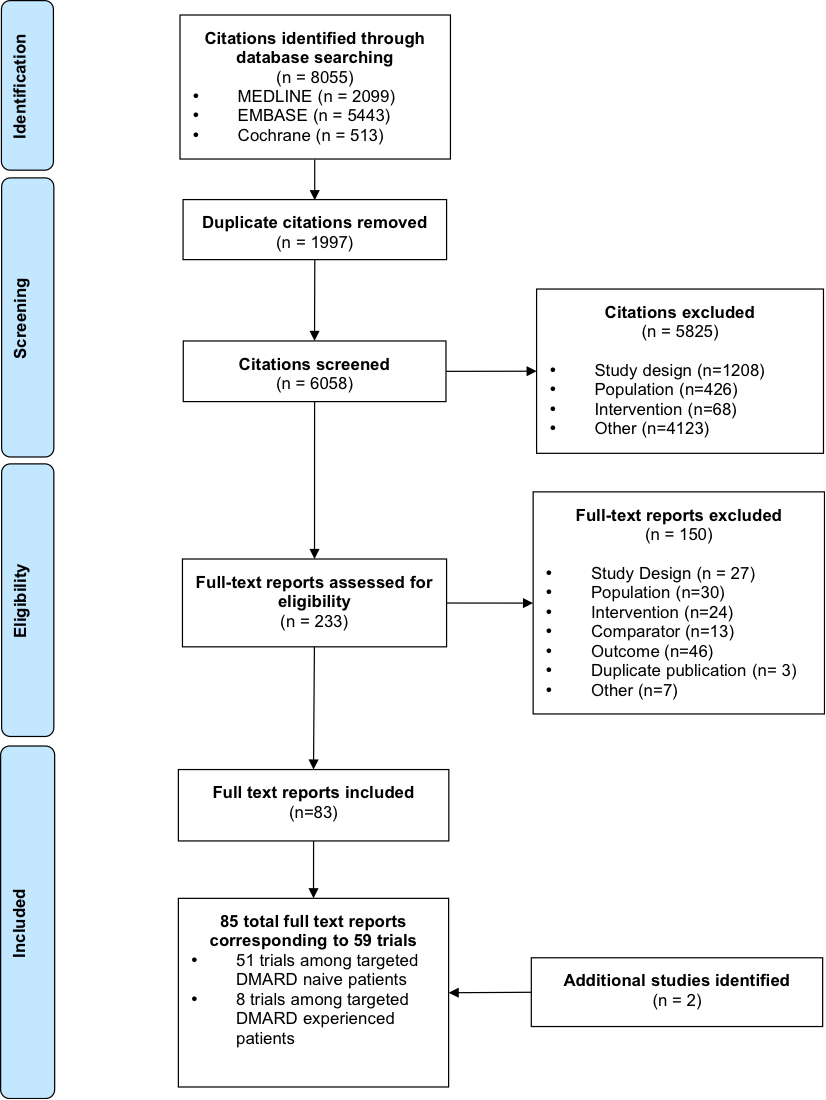
\includegraphics[max size={\textwidth}{\textheight}]{study-selection.png}
% \caption{Study identification and selection}\label{fig:study-selection}
% \end{figure}

% \begin{figure}
% \centering
% 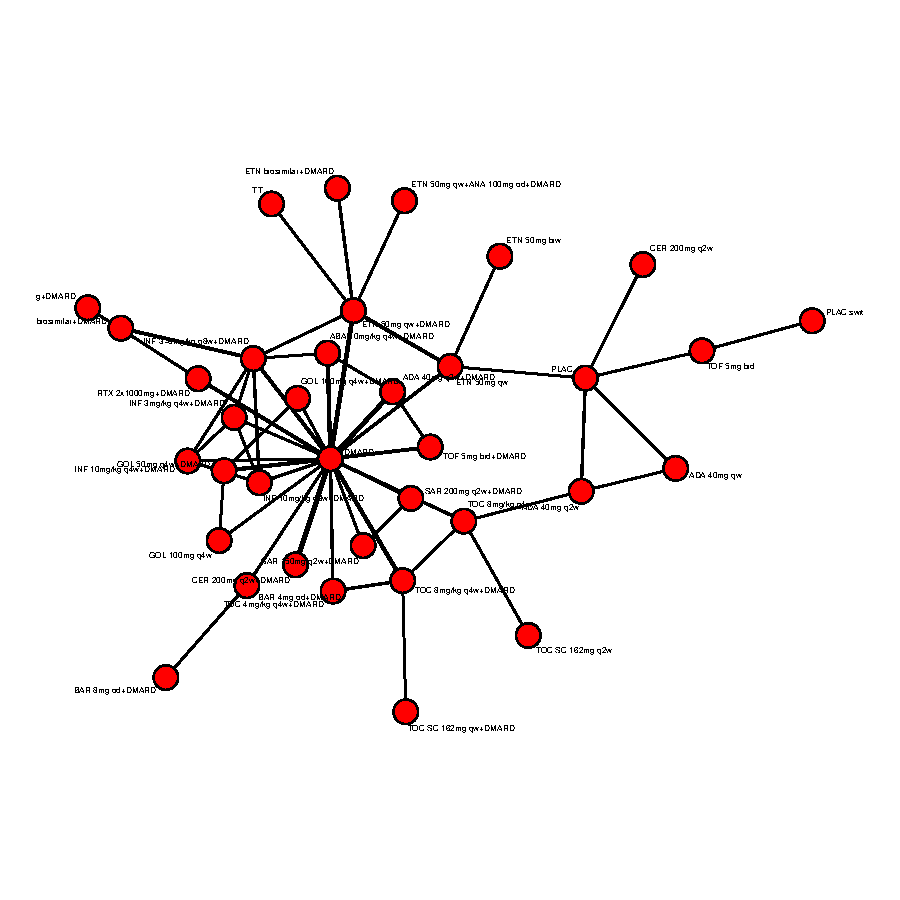
\includegraphics{nma-network-acr-naive.pdf}
% \caption{Bayesian random effects NMA network diagram for patients naive
% to bDMARDs}\label{fig:nma-network-acr-naive}
% \end{figure}

\subsection{Statistical models for network-meta analysis}\label{app:nma-statistical-models}

ACR response, 6 month change in HAQ from baseline, and 6 month change in DAS28 from baseline were estimated using a Bayesian (random effects) network meta-analysis approach. The four mutually exclusive ACR response categories were estimated using a ordered probit model appropriate for ordered categorical data \citep{dias2013evidence}. The model assumes that there is an underlying continuous variable (ACR20/50/70) categorized by specifying different cutoffs corresponding to the point at which an individual moves from one category to the next in each trial. The advantage of this approach over an analysis that considers ACR categories separately is that all possible outcomes are analyzed simultaneously based on the same randomized controlled trials, allowing for consistent estimates by category. The relative treatment effects for each bDMARD versus cDMARDs estimated on the probit scale were transformed into absolute probabilities of the non overlapping ACR response categories by combining them with the average results for cDMARDs.

Changes in HAQ and DAS28 from baseline at 6 months were estimated using a Bayesian (random effects) network meta-analyses model for continuous data \citep{dias2013evidence}. The models use a normal likelihood (since the sample mean is approximately normally distributed by the central limit theorem if the sample size is reasonably large) and an identity link. 

To avoid influencing the observed results by prior belief, uninformative prior distributions were used for the estimated model parameters. The posterior distributions of parameters of interest were summarized by the mean as a reflection of the point estimate and 95\% credible intervals, constructed from the 2.5 and 97.5 percentiles. Analyses were performed with the Markov chain Monte Carlo method using the JAGS software package (\url{http://mcmc-jags.sourceforge.net/}).

\subsection{Comparing the IVI NMA to the NICE NMA}\label{app:nma-ivi-nice-comp}
To help ensure that differences in cost-effectiveness estimates from our model relative to others are not driven by the NMA results, we compared our NMA estimates to estimates reported by NICE in \citet{stevenson2016adalimumab}. We focus on ACR response, since the NICE report and other models use treatment pathways similar to \textbf{H1} and \textbf{H2} and rarely use DAS28 to inform treatment duration. As shown in \autoref{tbl:nma-acr-nice-vs-ivi}, our results are similar and the NICE point estimates are generally within the 95\% credible intervals surrounding our point estimates.

\begin{table}[!ht]
\begin{center}
\scriptsize
\begin{threeparttable}
\caption{A comparison of NICE and IVI estimates of ACR response probabilities} \label{tbl:nma-acr-nice-vs-ivi}
\begin{tabularx}{\textwidth}{@{\extracolsep{\fill}}lrrrrrr}
\hline
\multicolumn{1}{c}{} & \multicolumn{3}{c}{IVI} & \multicolumn{3}{c}{NICE}\\
\cmidrule(lr){2-4} \cmidrule(lr){5-7}
\multicolumn{1}{l}{} & \multicolumn{1}{c}{ACR20} & \multicolumn{1}{c}{ACR50} & \multicolumn{1}{c}{ACR70} & \multicolumn{1}{c}{ACR20} & \multicolumn{1}{c}{ACR50} & \multicolumn{1}{c}{ACR70}\\
\hline
\ExpandableInput{tables/nma-acr-nice-vs-ivi.txt}
\hline
\end{tabularx}
\scriptsize
Notes: ACR20/50/70 categories are the probability of at least a 20/50/70\% improvement. 95\% credible intervals are in parentheses. IVI estimates are based on 6-month simulations of 1,000 patients and 1,000 parameters sets for each therapy. NICE estimates are from Table 37 in \citet{stevenson2017cost}. cDMARDs = conventional disease-modifying antirheumatic drugs; MTX = methotrexate; ABT IV = abatacept intravenous; ADA = adalimumab; ETN = etanercept; GOL = golimumab; IFX = infliximab; TCZ = tocilizumab; CZP = certolizumab pegol; ABT SC = abatacept subcutaneous; RTX = rituximab; TOF = tofacitinib. ACR = American College of Rheumatology.
\end{threeparttable}
\end{center}
\end{table}

\end{appendices}

\pdfbookmark[1]{References}{References}
\bibliography{../../vignettes/vignettes}

\end{document}
